\documentclass{ieeeaccess}
\usepackage{cite}
\usepackage{amsmath,amssymb,amsfonts}
\usepackage{algorithmic}
\usepackage{graphicx}
\usepackage{textcomp}
\usepackage{algorithm}
\usepackage{algpseudocode}
\usepackage{multirow}
\usepackage{booktabs}
\usepackage{color, soul}
\usepackage{subcaption}

\usepackage{bm}
\makeatletter
\AtBeginDocument{\DeclareMathVersion{bold}
\SetSymbolFont{operators}{bold}{T1}{times}{b}{n}
\SetSymbolFont{NewLetters}{bold}{T1}{times}{b}{it}
\SetMathAlphabet{\mathrm}{bold}{T1}{times}{b}{n}
\SetMathAlphabet{\mathit}{bold}{T1}{times}{b}{it}
\SetMathAlphabet{\mathbf}{bold}{T1}{times}{b}{n}
\SetMathAlphabet{\mathtt}{bold}{OT1}{pcr}{b}{n}
\SetSymbolFont{symbols}{bold}{OMS}{cmsy}{b}{n}
\renewcommand\boldmath{\@nomath\boldmath\mathversion{bold}}}
\makeatother

\def\BibTeX{{\rm B\kern-.05em{\sc i\kern-.025em b}\kern-.08em
    T\kern-.1667em\lower.7ex\hbox{E}\kern-.125emX}}

%Your document starts from here ___________________________________________________
\begin{document}
\history{Date of publication xxxx 00, 0000, date of current version xxxx 00, 0000.}
\doi{10.1109/ACCESS.2024.0429000}

\title{Modular Patch-Level Image Obfuscation Framework for Untrusted Third-Party Vision Inference}
\author{\uppercase{Jinmyeong Shin}\authorrefmark{1}, and
\uppercase{Yoon-Ho Choi}\authorrefmark{1,2},\IEEEmembership{Member, IEEE}}

\address[1]{Cloud Security Research Center, Pusan National University, Busan 46241, Republic of Korea}
\address[2]{School of Computer Science and Engineering, Pusan National University, Busan 46241, Republic of Korea}
\tfootnote{This work was supported by the Institute of Information \& Communications Technology Planning \& Evaluation (IITP) through the Information Technology Research Center (ITRC) program, funded by the Ministry of Science and ICT, Korea (IITP-2025-RS-2023-00259967). This work was also supported by the National Research Foundation of Korea (NRF) grant funded by the Korea government (MSIT) (No. RS-2023-00217689).}

\markboth
{J. Shin \headeretal: Modular Patch-Level Image Obfuscation Framework for Untrusted Third-Party Vision Inference}
{J. Shin \headeretal: Modular Patch-Level Image Obfuscation Framework for Untrusted Third-Party Vision Inference}

\corresp{Corresponding author: Yoon-Ho Choi (e-mail: yhchoi@pusan.ac.kr).}


\begin{abstract}
This paper presents a modular patch-level image obfuscation framework for privacy-preserving vision inference on untrusted third-party servers using Vision Transformer (ViT)--based architectures. The proposed framework applies client-side, non-invertible, channel-wise patch-level transformations that convert input images into visually unrecognizable forms while preserving the high-level semantic structure required by ViT patch embeddings. A lightweight server-side deobfuscator network approximates ViT-compatible embeddings directly from obfuscated inputs, thereby eliminating the need for raw image reconstruction and enabling seamless integration with frozen pretrained transformer backbones. In addition, the framework incorporates a Merkle tree--based attestation mechanism for execution integrity verification and supports randomized obfuscation scheduling to strengthen resilience against reconstruction attacks. The framework is evaluated across diverse vision tasks including classification, zero-shot recognition, optical character recognition, object detection, and medical image analysis. Experimental results demonstrate that the proposed method maintains high task utility with minimal performance degradation: over 98\% top-1 accuracy on CIFAR-10, over 92\% word-level F1-score on OCR, and consistent performance on medical imaging benchmarks. Moreover, empirical security evaluations using MI-FGSM, L-BFGS inversion, adversarial VAE, and side-channel leakage analyses confirm robust resistance to reconstruction attacks. Each deobfuscator is trained in under five minutes, confirming the framework's efficiency and suitability for practical deployment in privacy-sensitive vision applications.
\end{abstract}

\begin{keywords}
Privacy-Preserving Deep Learning, Vision Transformer, Data Privacy, Cloud Computing Environment
\end{keywords}

\titlepgskip=-21pt

\maketitle

\section{Introduction} \label{sec:intro}

\PARstart{I}{n} recent years, deep learning based vision models have demonstrated exceptional performance across a wide range of visual recognition tasks, including classification, detection, and retrieval~\cite{VoulodimosDeep2018, CHAI2021100134, Alsajri_Hacimahmud_2023, TSIRTSAKIS2025298}. However, deploying such models in real-world systems, particularly cloud-based inference system, introduces serious privacy concerns. In domains such as medical image analysis, industrial inspection, and surveillance analytics, raw image data often contains sensitive information that cannot be exposed to unauthorized parties due to legal, ethical, or strategic constraints~\cite{Grünberg2017,info:doi/10.2196/22269, Padmapriya2024, 01630814-202314060-00005, app132312727}.

A promising method to mitigate such risks is to obfuscate visual content before it is transmitted or processed externally. Most of existing methods rely on learned encryption schemes~\cite{TANWAR2022103503,10.1145/3570165,Madani_2025} or autoencoder-based pipelines~\cite{s23010519,Zhou2024,SHIRI2024104583,10781629} that reconstruct either full-resolution original image or compressed representations which is very similar to original visual content at the service end. While effective at reducing raw data exposure, these approaches tightly couple the encoder and decoder, requiring both components to be deployed together. This not only increases the model size and inference latency but also poses a security risk that the full original image reconstruction is possible when the decoder is compromised.

In addition, there are some researches about image data obfuscation method that is free from the compromised decoder~\cite{9129656,10.1007/978-3-031-37586-6_18,s24103166}, but those methods require huge computation costs for re-training with obfuscated images. Also, Since they showed the feasibility of each method in a specific classification task, their generalizability across broader vision tasks such as detection, segmentation, or retrieval remains limited. Moreover, their tight coupling between obfuscation and task-specific re-training hinders modular deployment, making them less practical for scalable or plug-and-play secure inference pipelines.

To address these limitations, we propose a modular and lightweight privacy-preserving framework that supports secure inference on untrusted or semi-trusted infrastructures such as public clouds. The framework introduces a non-invertible, patch-level channel obfuscation method executed on the client side, which disrupts local visual statistics while preserving the high-level semantic features necessary for machine recognition.

To achieve compatibility with existing vision transformer~(ViT)-like patch embedding architectures~\cite{dosovitskiy2020vit}, we employ a compact deobfuscator network that approximates the output of the original ViT's patch embedding layer, generating token embeddings directly from the obfuscated image. ViT-like patch embedding techniques have become widely adopted in state-of-the-art multi-modal large language models (LLMs), since GPT-4 by OpenAI~\cite{2023GPT4VisionSC}, Google's Gemini~\cite{geminiteam2025geminifamilyhighlycapable}, Meta's Llma 3.2~\cite{meta2024llama3} and NVIDIA's NVLM~\cite{dai2024nvlmopenfrontierclassmultimodal}. By aligning our design with this widely adopted embedding format, our approach ensures easy and practical integration into existing transformer-based inference pipelines. In addition, this approach separates obfuscation-deobfuscation stage, which is privacy-sensitive, from the ViT backbone network. Therefore, the model does not need to reconstruct the original image or any visual output. Instead, it focuses only on features needed for recognition tasks. This is a key difference from autoencoder-based methods, which reconstruct the original or similar image for further processing.

In addition to the obfuscation and deobfuscation modules, the framework is architected to ensure the integrity and authenticity of inference execution. It enables clients to verify that only authorized model configurations are used during inference, without relying on trusted infrastructure or secure hardware. Also, the system also embraces a simple yet powerful architectural principle: introducing variability in obfuscation paths at runtime. By selecting from a set of interchangeable obfuscators during deployment, it disrupts consistent transformation patterns and significantly increases resistance to inversion and approximation attacks

We evaluate the proposed system across a range of vision tasks using ViT-based models, including classification, zero-shot recognition, OCR, object detection, and medical image analysis. The framework maintains high utility, achieving over 98\% top-1 accuracy on CIFAR-10 and over 92\% word-level F1 score on OCR benchmarks, with consistent performance on medical imaging tasks. We further validate robustness through adversarial evaluations including MI-FGSM, L-BFGS inversion, adversarial VAE, and side-channel leakage analysis. The lightweight deobfuscators can be trained in under 5 minutes, underscoring the framework's practicality for deployment scenarios.

The contributions of this paper can be summarized as follows:
\begin{itemize}
    \item \textbf{Privacy-preserving image obfuscation and deobfuscation architecture:} We propose a non-invertible, channel-wise patch-level obfuscation scheme applied entirely on the client side. This transformation irreversibly removes low-level visual features while preserving high-level semantics, enabling downstream inference without exposing human-recognizable content. A lightweight deobfuscator reconstructs ViT-compatible embeddings without requiring access to the original image
    \item \textbf{Modular architecture compatible with ViT models:} The framework is designed to operate independently of the ViT backbone. The deobfuscator is trained to match frozen transformer patch embeddings, enabling plug-and-play compatibility with standard pretrained models such as CLIP and GPT-4V without requiring retraining or architectural modification.
    \item \textbf{Secure inference on untrusted third-party infrastructures with Merkle attestation:} To ensure execution integrity, the framework incorporates a Merkle tree–based attestation mechanism. This allows clients to cryptographically verify that inference is conducted using authorized model components, even when deployed on untrusted third-party servers.
\end{itemize}

The remainder of this paper is organized as follows. Section~\ref{sec:rel} reviews related work. Section~\ref{sec:threat-model} presents the threat model. Section~\ref{sec:pro} details the proposed framework. Section~\ref{sec:sec} provides a security analysis, and Section~\ref{sec:exp} presents experimental results. Section~\ref{sec:con} concludes the paper.

% ===================================================================================
\section{Related Works} \label{sec:rel}

\begin{table*}[!t]
\caption{\textbf{Comparison of the Proposed Method with Existing ViT-Based Privacy-Preserving Vision Inference Methods}}
\label{tab:method-comparison}
\centering
\begin{tabular}{@{}p{0.15\textwidth} p{0.19\textwidth} p{0.18\textwidth} p{0.18\textwidth} p{0.18\textwidth}@{}}
\toprule
\textbf{Feature} & \textbf{Proposed Method} & \textbf{Hao et al.~\cite{hao2023privacypreserving}} & \textbf{Feng et al.~\cite{10445482}} & \textbf{Horio et al.~\cite{horio2024privacypreservingvisiontransformerusing}} \\
\midrule

\textit{Architecture Type} &
Modular obfuscation--deobfuscation with ViT embedding interface &
Permutation-equivariant ViT trained on shuffled/mixed encrypted inputs &
JPEG-encrypted feature extraction with ViT-based retrieval model &
ViT fine-tuning on permuted encrypted images \\
\midrule

\textit{Privacy Mechanism} &
Randomized Conv2D + dual permutation + randomized obfuscator scheduling &
Random Shuffling (RS) + Mixing (MI) of image sub-patches &
JPEG DCT stream cipher + handcrafted image-level features &
Block/pixel permutation with shared random matrix key \\
\midrule

\textit{Inference Attestation} &
\checkmark~Merkle tree--based attestation on untrusted infrastructure &
$\times$~Not addressed &
$\times$~Not addressed &
$\times$~Not addressed \\
\midrule

\textit{Training Time} &
$<$10 minutes (deobfuscator only) &
$>$2 hours (custom ViT/YOLOS variants) &
$>$3 hours (ViT + feature training) &
$>$2 hours (full ViT fine-tuning) \\
\midrule

\textit{Compatibility with ViTs} &
\checkmark~Directly compatible with frozen ViTs (e.g., CLIP, GPT-4V) &
$\times$~Requires permutation-equivariant redesign of ViT &
$\times$~Requires retraining of modified ViT &
$\times$~Requires retraining of ViT backbone \\
\midrule

\textit{Retraining Impact on ViT-based Models} &
\checkmark~No retraining needed for downstream ViT-based models &
$\times$~Must redesign all dependent ViT components &
$\times$~Incompatible with standard pretrained ViT pipelines &
$\times$~All ViT-based models must be retrained on permuted data \\
\bottomrule
\end{tabular}
\end{table*}

{In recent years, privacy-preserving image analysis methods have received considerable attention due to growing concerns regarding the protection of sensitive visual information in cloud-based services. The approaches to address these concerns can be broadly categorized into two distinct paradigms: (1) \textit{to protect the data during model training-time} and (2) \textit{to protect data during inference-time}.

The first paradigm, training-time privacy, aims to protect the confidentiality of the data within the training dataset itself. Approaches such as secure multi-party computation~(SMPC), and methods based on differential privacy, which can be represented with DP-SGD}~\cite{Abadi_2016}{ and PATE}~\cite{46614}{, and federated learning are designed to produce a final model that does not leak significant information about any individual training example. While these methods provide strong, often formal, privacy guarantees, they frequently introduce "impossible computational overhead for practical deployment" or require significant, costly model retraining.

The second paradigm, inference-time privacy, addresses the threat of data exposure when a user sends their private data to a third-party server for analysis with a pre-trained model. The goal is to make the user's data unintelligible to the server while preserving its utility for the specific task. Existing approaches for inference-time privacy primarily fall into two categories: \textit{encryption-based schemes} and \textit{autoencoder-based methods}, each with distinct trade-offs in security, computational cost, and applicability.}

\subsection{Learned Encryption Schemes}

Encryption-based privacy-preserving methods generally rely on cryptographic algorithms or learnable encryption techniques to obfuscate image data before transmission or processing. For example, Tanwar et al.~\cite{TANWAR2022103503} introduced a permutation-ordered binary number encryption approach specifically designed for cloud-based deep learning image recognition tasks. While achieving strong security guarantees, their method involves computationally expensive operations and often suffers from high inference latency due to encryption overheads.

Ahmed et al.\cite{10.1145/3570165} proposed a DNA-based image encryption method combined with convolutional autoencoders and chaotic sequences, effectively reducing the dimensionality of input images and securing them via encryption. Although their technique demonstrates robustness against various attacks, the coupling of encryption with dimensionality reduction increases model complexity, complicating deployment in real-time or lightweight scenarios. Madani and Bourennane\cite{Madani_2025} presented a CNN-based autoencoder integrated with visual encryption, but their method required both the encoder and decoder to reside at the service provider, potentially exposing sensitive reconstruction components. Nagamori et al.~\cite{jimaging8090233} introduced a privacy-preserving semantic segmentation approach, where images undergo block-wise encryption before being fed to the segmentation model. Their method successfully preserved visual privacy while retaining high segmentation accuracy; however, similar to other encryption-based approaches, the computational complexity introduced by encryption remained significant, presenting challenges for real-time applications.

Furthermore, encryption-based methods leveraging homomorphic encryption and secure multi-party computation~(SMPC), as presented by many researchers~\cite{9936637,9833432,Jia2023,refId0,10.1145/3676641.3716008,garimella2025helrmencrypteddeeplearning,dhyani2023privitvisiontransformersfast,luo-etal-2024-secformer}, ensure strong theoretical guarantees but introduce impossible computational overhead for practical deployment in real-world scenarios.

\subsection{Autoencoder-Based Obfuscation Methods}

Autoencoder-based approaches attempt to protect privacy by encoding images into compressed, latent representations that can be reconstructed at the service end. Shiri et al.\cite{SHIRI2024104583} introduced a privacy-preserving medical image sharing framework using sparse representation learning. Although effective in reducing image redundancy, their method involves reconstructing images from sparse representations, which inherently risks information leakage if the reconstruction model is compromised. Zhou et al.\cite{Zhou2024} developed a synthetic data generation pipeline utilizing autoencoders to enhance privacy in medical image diagnosis. This approach, while beneficial for privacy protection during training, again relies on the careful deployment of both encoder and decoder at the service provider’s side.

Sirisha and Chandana~\cite{s23010519} proposed a secure deep-learning framework integrating image encryption and accident severity classification via convolutional autoencoders and YOLO-based object detection. While successfully mitigating privacy concerns in accident image management scenarios, the complexity introduced by integrated autoencoder structures increased computational requirements and inference latency. Additional work by Naveen et al.~\cite{10781629} proposed an autoencoder-based image compression scheme tailored to reduce the bandwidth needed for secure data transmission, although reconstruction at the cloud side still posed privacy risks if compromised.

\subsection{Decoder-Free Obfuscation Methods}

% \begin{table*}[t]
% \centering
% \caption{Comparison of the Proposed Method with Existing ViT-Based Privacy-Preserving Vison Inference Methods.}
% \label{tab:method-comparison}
% \begin{tabular}{>{\raggedright\arraybackslash}p{0.14\textwidth}
%                 >{\raggedright\arraybackslash}p{0.19\textwidth}
%                 >{\raggedright\arraybackslash}p{0.18\textwidth}
%                 >{\raggedright\arraybackslash}p{0.18\textwidth}
%                 >{\raggedright\arraybackslash}p{0.18\textwidth}}
% \toprule
% \textbf{Feature} & \textbf{Proposed Method} & \textbf{Hao et al.~\cite{hao2023privacypreserving}} & \textbf{Feng et al.~\cite{10445482}} & \textbf{Horio et al.~\cite{horio2024privacypreservingvisiontransformerusing}} \\
% \midrule

% \textit{Architecture Type} &
% Modular obfuscation– deobfuscation with ViT embedding interface &
% Permutation-equivariant ViT trained on shuffled/mixed encrypted inputs &
% JPEG-encrypted feature extraction with ViT-based retrieval model &
% ViT fine-tuning on permuted encrypted images \\

% ine

% \textit{Privacy Mechanism} &
% Randomized Conv2D + dual permutation + randomized obfuscator scheduling &
% Random Shuffling (RS) + Mixing (MI) of image sub-patches &
% JPEG DCT stream cipher + handcrafted image-level features &
% Block/pixel permutation with shared random matrix key \\

% ine

% \textit{Inference Attestation} &
% \checkmark~Merkle tree–based attestation on untrusted infrastructure &
% $\times$ Not addressed &
% $\times$ Not addressed &
% $\times$ Not addressed \\

% ine

% \textit{Training Time (per model)} &
% $<$5 minutes (deobfuscator only) &
% $>$2 hours (custom ViT/YOLOS variants) &
% $>$3 hours (ViT + feature training) &
% $>$2 hours (full ViT fine-tuning) \\

% ine

% \textit{Compatibility with Existing ViTs} &
% \checkmark~Directly compatible with frozen ViTs (e.g., CLIP, GPT-4V) &
% $\times$ Requires permutation-equivariant redesign of ViT &
% $\times$ Requires retraining of modified ViT &
% $\times$ Requires retraining of ViT backbone \\

% ine

% \textit{Retraining Impact on ViT-based Models} &
% \checkmark~No retraining needed for downstream ViT-based models &
% $\times$ Must redesign all dependent ViT components &
% $\times$ Incompatible with standard pretrained ViT pipelines &
% $\times$ All ViT-based models must be retrained on permuted data \\

% \bottomrule
% \end{tabular}
% \end{table*}

Recently, a new direction emerged focusing on obfuscation strategies that eliminate the need for image reconstruction at the cloud provider, thereby removing the threat associated with compromised decoders. Ko et al.~\cite{9129656} presented a structural image de-identification approach that obfuscates identity-sensitive features in images. However, their method demanded substantial computational resources for re-training models on structurally modified images, limiting its practicality. Rodriguez and Krishnan~\cite{10.1007/978-3-031-37586-6_18} developed an autoencoder-based image anonymization scheme explicitly designed to preserve non-sensitive features while removing identifiable attributes. Although effective within specific classification tasks, their method required extensive task-specific retraining for each new application scenario, hindering modularity and scalability.

Kim et al.~\cite{s24103166} introduced a differential privacy-based image generation method leveraging dual noise mechanisms for obfuscation, making images unrecognizable to humans but useful for machine analysis. Despite achieving privacy guarantees, the method's applicability remained restricted to classification tasks, and significant computational overhead for re-training models with privacy-preserving noise was required. Moreover, Popescu et al.~\cite{9786187} proposed image obfuscation algorithm based on pixel intensity shuffling and non-bijective functions, but their solutions faced similar computational burdens and limited generalizability beyond classification contexts. Oh et al.~\cite{oh2022differentially} presented a differentially private approach called DP-CutMixSL for split learning with Vision Transformers, combining patch-level CutMix augmentations and differential privacy mechanisms. While effective in enhancing resistance to membership inference attacks, their method was primarily optimized for split-learning scenarios and still required careful retraining of models with privacy-specific augmentations, thereby maintaining certain scalability and deployment constraints.

Beyond these task-specific methods, the broader adversarial robustness literature has highlighted fundamental privacy risks in deep learning systems. Zhu et al.~\cite{zhu2019deep_leakage} demonstrated that training data can be reconstructed from shared gradients, motivating inference-time privacy solutions. Carlini et al.~\cite{carlini2021extracting} showed that large models can memorize and leak training data, underscoring the need for privacy-preserving inference even when models are frozen. Recent work on differentially private Vision Transformers~\cite{he2024diff_privacy_vit} has explored applying DP noise at the token level, but these approaches trade significant accuracy for privacy guarantees and require model retraining. The emergence of hierarchical ViT architectures such as Swin Transformer~\cite{liu2021swin} and SegFormer~\cite{xie2021segformer} has further expanded the design space for privacy-preserving vision systems, as these models process visual information at multiple scales.

With the rise of ViT-like architectures, recent studies have begun exploring transformer-specific privacy-preserving methods. Hao et al.~\cite{hao2023privacypreserving} introduced a secure ViT architecture integrated with privacy-preserving mechanisms at token-level encryption, but the method relied heavily on retraining the ViT backbone and complicated the training pipeline. Similarly, Feng et al.~\cite{10445482} presented a ViT-based privacy framework utilizing multi-layered encryption at images and Huffman-Code frequency at embedding layers, increasing computation costs and training complexity. Horio et al.~\cite{horio2024privacypreservingvisiontransformerusing} proposed a permutation-based encryption method for ViTs using fixed random matrices, but it also required ViT retraining and lacked compatibility with frozen pretrained models.





\\

Compared to existing methods~\cite{hao2023privacypreserving,10445482,horio2024privacypreservingvisiontransformerusing}, the proposed method offers a modular, client-side obfuscation scheme based on non-invertible channel-wise patch-level transformations. As summarized in Table~\ref{tab:method-comparison}, it is the only framework that supports seamless integration with frozen ViT models, avoiding the need for retraining or architectural changes. The deobfuscator can be trained efficiently in under five minutes and operates independently of the obfuscator and backbone. Additionally, the framework introduces Merkle tree–based inference attestation, ensuring verifiable execution integrity even on untrusted servers. These capabilities collectively enable secure, scalable, and efficient deployment for privacy-preserving vision tasks in real-world settings.


% Compared to existing methods~\cite{hao2023privacypreserving,10445482,horio2024privacypreservingvisiontransformerusing}, proposed approach stands apart by adopting a modular, non-invertible patch-level obfuscation scheme applied client-side, decoupled entirely from the embedding and inference processes performed on the cloud. Our method eliminates the need for image reconstruction or any visually recognizable output at the service provider’s end, significantly reducing privacy risks associated with compromised decoder components. By introducing multiple obfuscation modules selectable at runtime, our architecture enhances robustness against inversion and reconstruction attacks without increasing substantial computational overhead. These design choices offer a scalable, efficient, and highly secure alternative for privacy-preserving inference services, applicable across diverse computer vision tasks including classification, retrieval, and detection, without requiring extensive task-specific retraining.

% ===================================================================================



\section{Threat Model}\label{sec:threat-model}

\begin{figure*}[t]
\centering
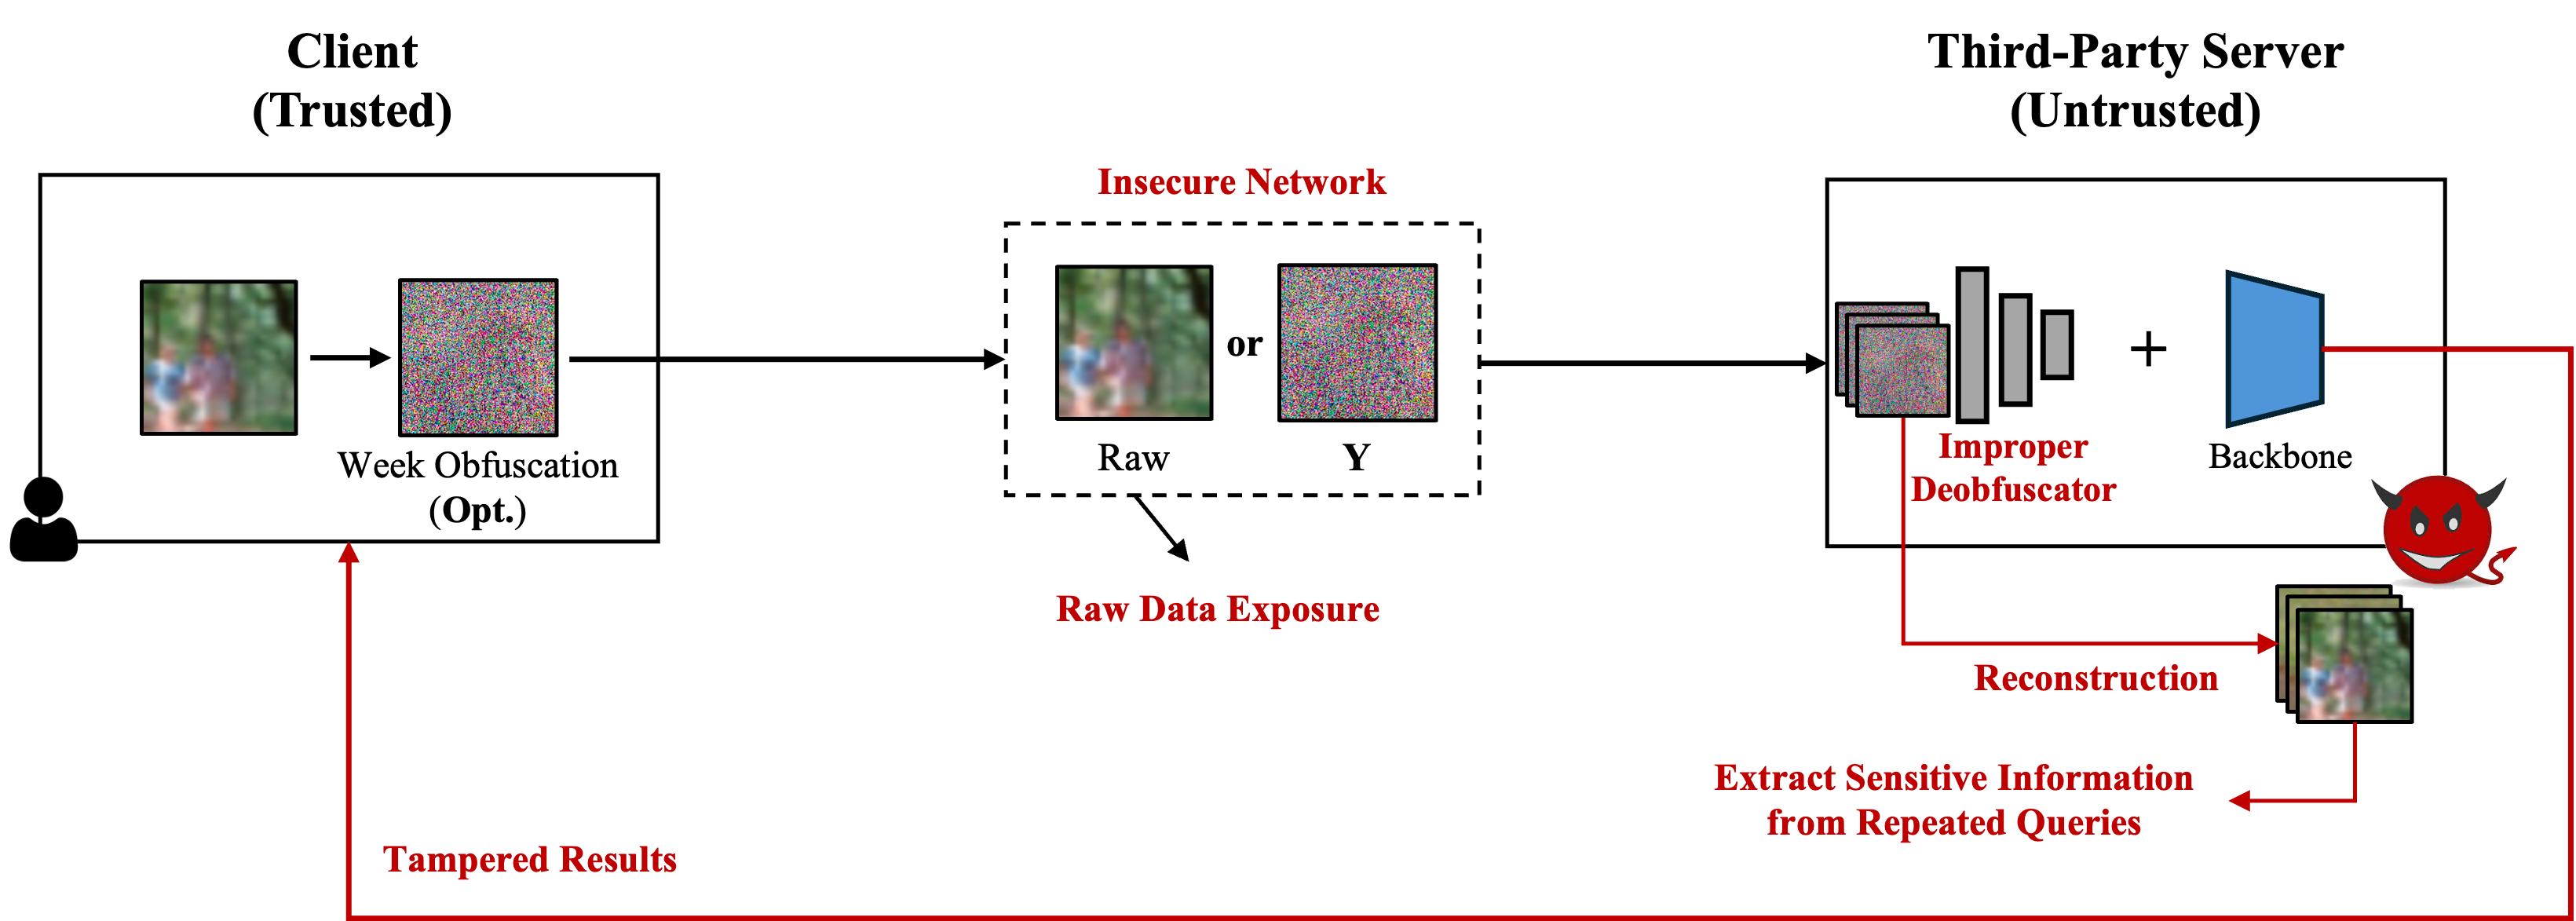
\includegraphics[width=0.8\linewidth]{figures/Threat Model.png} % Update path as needed
\caption{Threat model of privacy-preserving inference in untrusted environments. A client optionally applies weak obfuscation to the input image, which is then transmitted over an insecure network. The inference server, assumed to be untrusted, has full access to the deobfuscator and backbone model. This enables adversaries to attempt reconstruction of the original image, extract sensitive information through repeated queries, and tamper with model outputs. Without secure obfuscation and verifiable execution, both data confidentiality and integrity are at risk.}
\label{fig:threat-model}
\end{figure*}

This work targets privacy-preserving inference in scenarios where image processing and prediction are delegated to third-party servers that may not be fully trusted. In such deployments, the inference infrastructure, including model hosting and execution, is operated by a potentially curious or malicious service provider. As a result, we adopt a zero-trust threat model that prioritizes both data confidentiality and execution integrity without assuming the correctness of the server’s behavior.

{Our threat model assumes a strong adversary who operates under a white-box model for all server-side components but faces a black-box model for the client's private operations. As illustrated in Figure}~\ref{fig:threat-model}{, the adversary is the inference server itself. In this white-box context, the attacker has complete access to the deployed deobfuscator and backbone models, can inspect and log all obfuscated inputs and their corresponding outputs, and may attempt to derive inverse transformations or semantic reconstructions using adaptive machine learning techniques. The adversary may also attempt to tamper with the execution flow by substituting unauthorized model components. However, even with this extensive power on the server, the attacker's capabilities are strictly limited at the client boundary. The client-side obfuscator remains a secure black box, meaning the attacker does not have access to the original images before obfuscation, the obfuscator's internal parameters, or the cryptographic keys used to sign execution configurations. This fundamental separation ensures that the user's raw data and the transformation secrets remain confidential.}


To defend against this class of adversary, the system must achieve several core guarantees. First, it must ensure that input data cannot be feasibly reconstructed from its obfuscated form, even when the deobfuscator and backbone are fully exposed. Second, the inference server must not be able to forge or substitute model components without detection. Third, inference results must be provably tied to the correct inputs and configurations, preventing replay, forgery, or selective misbehavior. Finally, the system must resist adaptive attacks that exploit structural regularities or statistical consistencies across samples to approximate the obfuscation transformation.

These requirements motivate the design of a framework in which the obfuscation process is randomized and client-side, the deobfuscator is trained to reconstruct only model-compatible embeddings rather than pixel-level features, and the execution path is cryptographically attested using Merkle tree signatures and per-request bindings. The following section details the architecture and mechanisms used to meet these goals.

% ===================================================================================

\section{Proposed Framework \& Methods} \label{sec:pro}

\begin{figure*}[t]
    \centering
    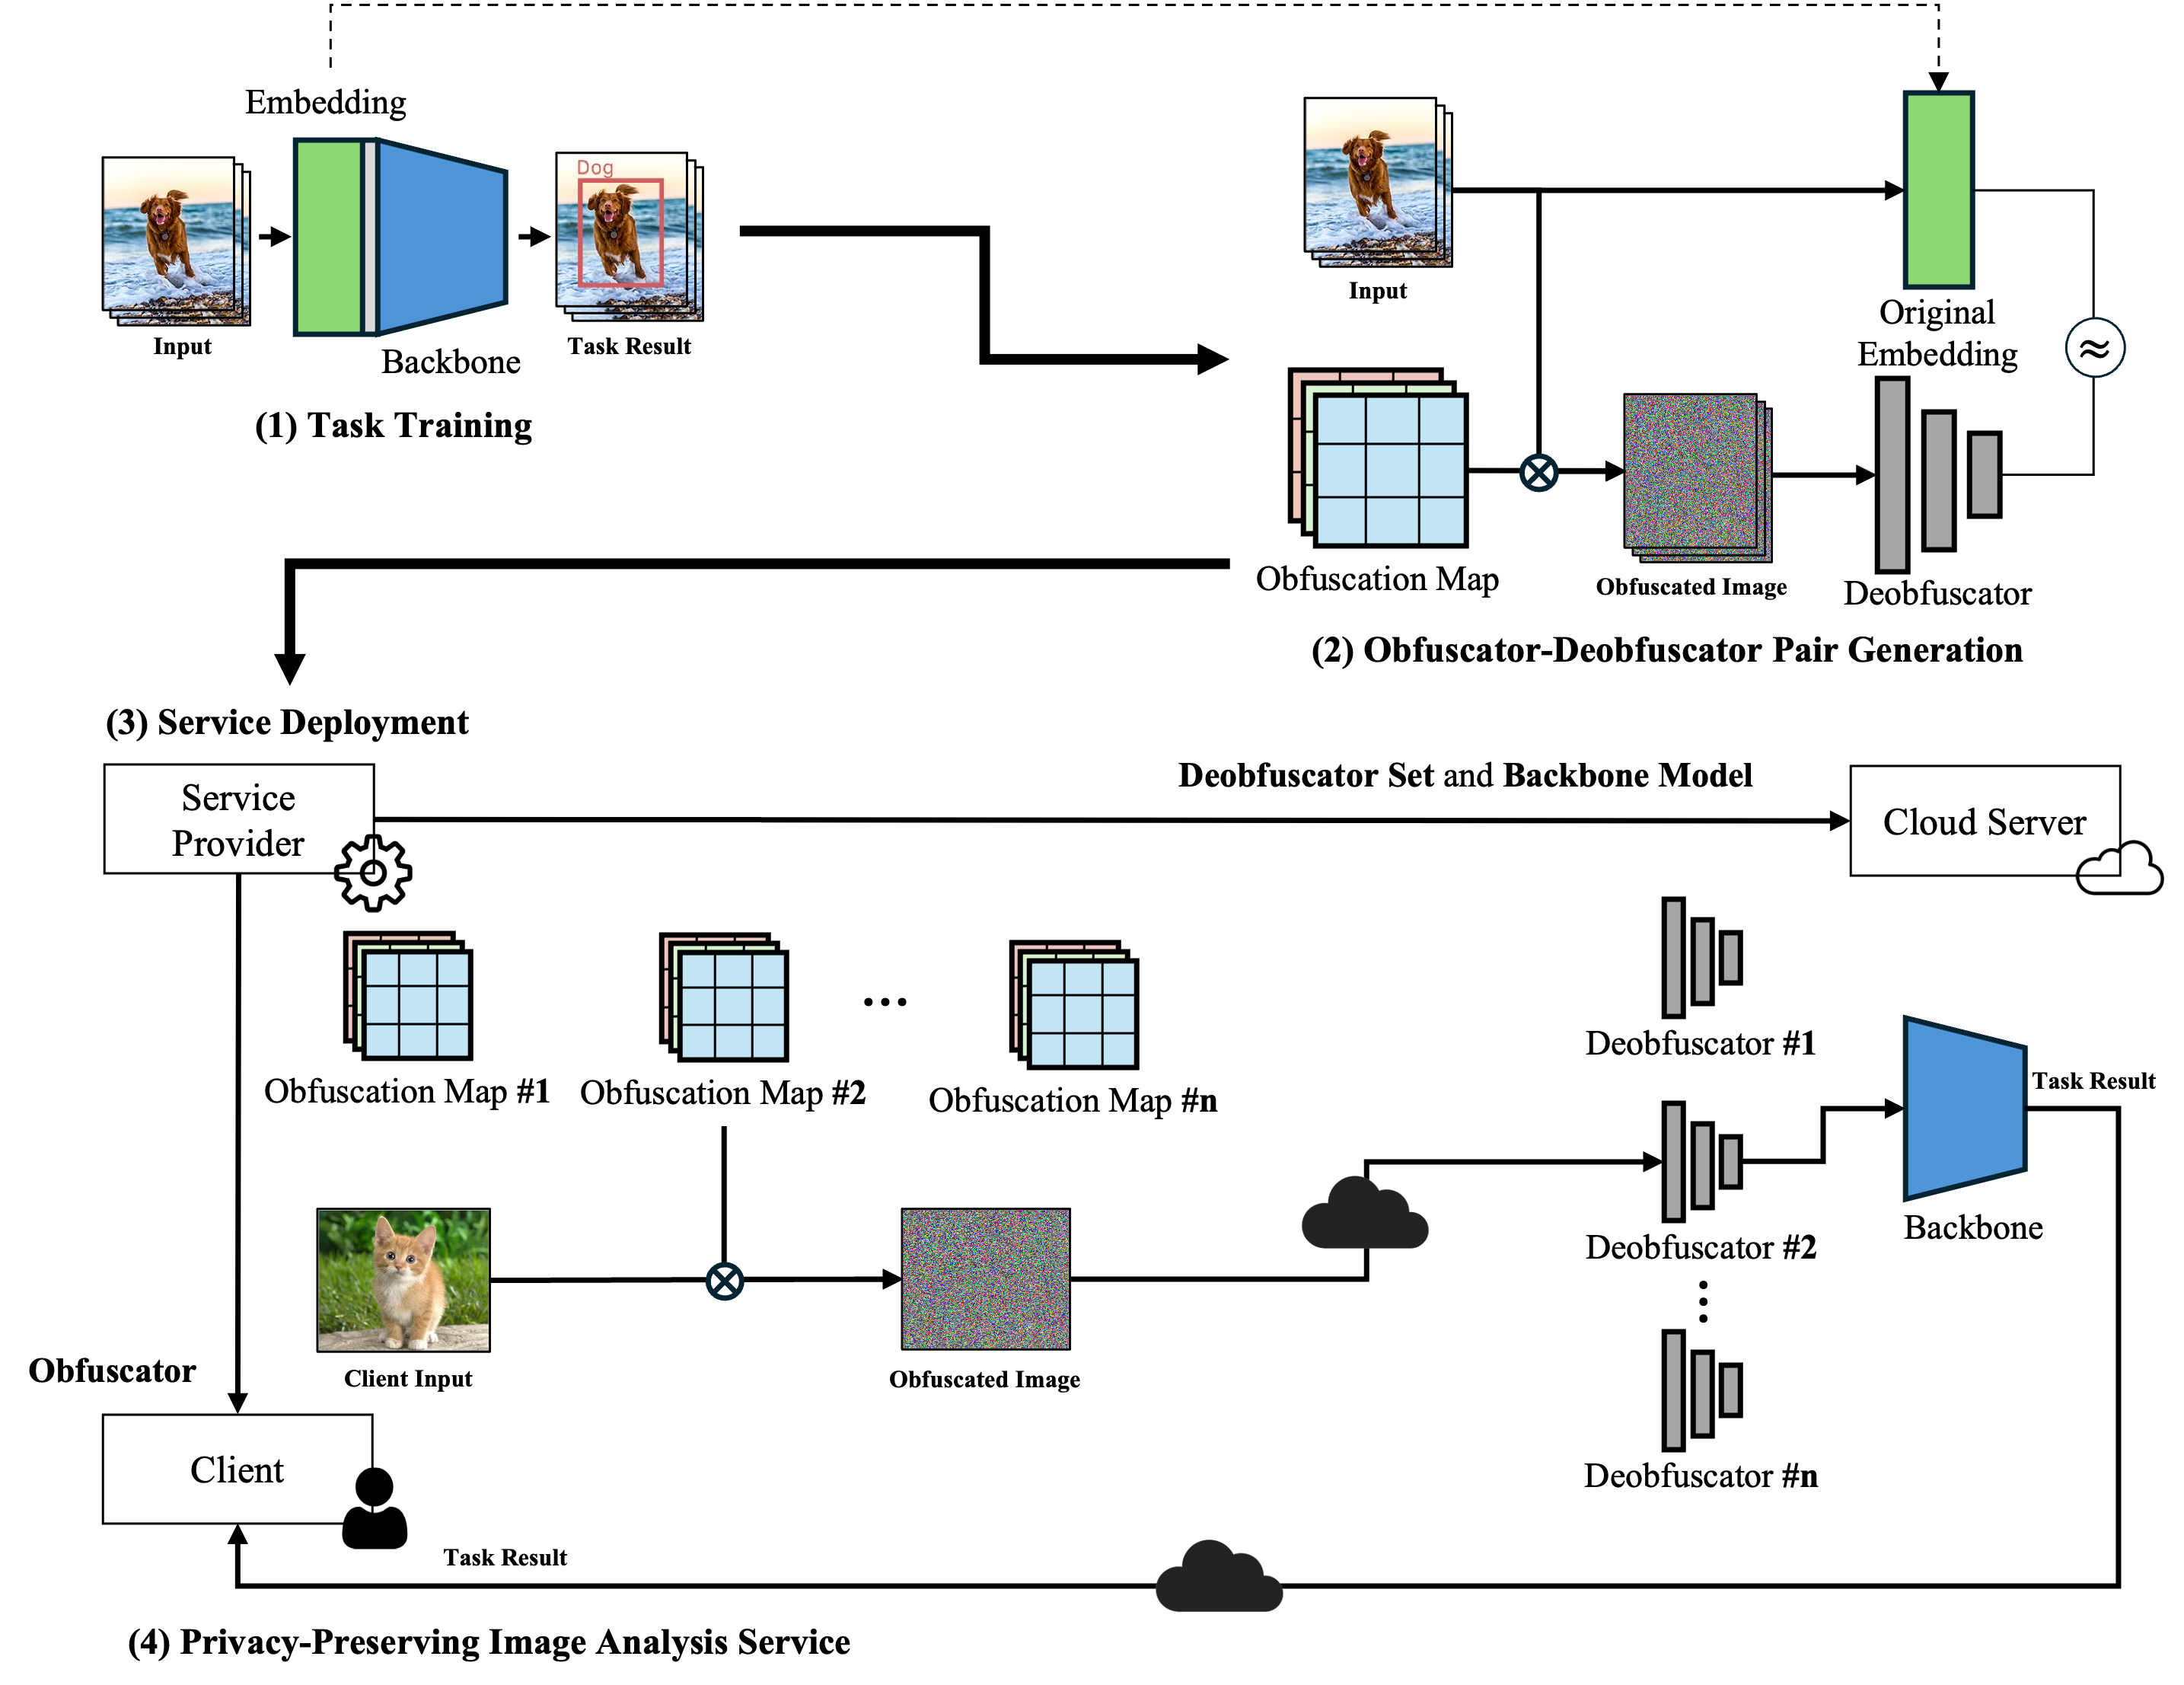
\includegraphics[width=0.8\linewidth]{figures/Overview.png}
    \caption{Overview of the proposed privacy-preserving image analysis framework. The system comprises a service provider, client-side obfuscation modules, and deobfuscation modules alongside a frozen transformer-based backbone hosted on an untrusted third-party inference server. The obfuscation modules remove low-level visual features from the input, while the deobfuscator reconstructs ViT-compatible embeddings without ever revealing or reconstructing the raw image content.}
    \label{fig:overview}
\end{figure*}

\subsection{Framework Overview} \label{sec:pro:overview}

% \renewcommand{\arraystretch}{1.1}
\begin{table}[t]
\centering
\caption{Summary of Notations}
\label{tab:notation-summary}
\begin{tabular}{p{0.05\textwidth} p{0.25\textwidth} p{0.10\textwidth}}
\toprule
\textbf{Symbol} & \textbf{Definition} & \textbf{Shape / Type} \\
\midrule
$X$ & Input image tensor & $\mathbb{R}^{C \times H \times W}$ \\
$Y$ & Obfuscated output tensor & $\mathbb{R}^{C \times H \times W}$ \\
$C$ & Number of channels (e.g., RGB: $C=3$) & Integer \\
$H, W$ & Height and width of the image & Integer \\
$p$ & Patch size (square: $p \times p$) & Integer \\
$P$ & Number of patch groups per channel & Integer \\
$W_{c,k}$ & Convolutional kernel for channel $c$, group $k$ & $\mathbb{R}^{1 \times p \times p}$ \\
$(i, j)$ & Top-left coordinate of a patch & Integer pair \\
$k$ & Patch group index, $k = \left( \frac{i}{p} \cdot \frac{W}{p} + \frac{j}{p} \right) \mod P$ & Integer \\
$Q$ & Obfuscated patch via $W_{c,k} * P$ & $\mathbb{R}^{p \times p}$ \\
$\pi_c$ & Patch permutation for channel $c$ & Permutation \\
$\rho$ & Global channel permutation map & Permutation \\
$f_i$ & Patch projection in deobfuscator & $\mathbb{R}^{p^2 \to d'}$ \\
$g_i$ & Channel fusion from $C \cdot d'$ to $D$ & $\mathbb{R}^{C \cdot d' \to D}$ \\
$D_\phi(Y)$ & Output embedding of deobfuscator & $\mathbb{R}^{B \times D \times H' \times W'}$ \\
$p_{\text{obf}}, p_{\text{deobf}}$ & Patch sizes for obfuscator and deobfuscator & Integers \\
$T_i$ & Configuration tuple: $(H_{\text{obf}}, H_{\text{deobf}}, H_{\text{backbone}})$ & Triple of hashes \\
$\text{Sig}_{\text{exec}}$ & Signature over inference tuple & Digital signature \\
\bottomrule
\end{tabular}
\end{table}

The proposed framework enables privacy-preserving image inference on untrusted or semi-trusted computational environments, such as cloud-based AI services. As shown in Figure~\ref{fig:overview}, the architecture involves three key entities: a service provider, a client, and a third-party inference server.

The service provider is responsible for offline model preparation. This includes training task-specific backbone models and generating a set of fixed, non-invertible obfuscation maps. Each obfuscation map is paired with a corresponding lightweight deobfuscator trained to approximate the output of a ViT patch embedding layer. Importantly, this deobfuscator is trained without ever accessing the original input images. This design ensures that the privacy of raw data is maintained, even if the server-side components are exposed.

The client serves as the trusted entry point to the system. It receives a signed set of obfuscation maps and applies one of them—selected either deterministically or at random—to the input image. The result is a visually unrecognizable obfuscated image, which retains sufficient high-level semantics for downstream model inference. The transformation is intentionally designed to be non-invertible, patch-level, and channel-wise, and requires only a few convolutional and permutation operations, making it highly efficient for edge deployment.

The third-party inference server, which is assumed to be untrusted, hosts only the task-specific frozen backbone and the pre-trained deobfuscator. Upon receiving the obfuscated input, the server applies the corresponding deobfuscator to recover ViT-compatible embeddings and proceeds with standard inference. Due to the decoupled architecture, the server cannot reconstruct or infer the original image, even if the deobfuscator and model weights are fully compromised.

To ensure integrity of the inference process, the framework includes a Merkle tree–based attestation mechanism. The service provider signs a root hash derived from all authorized (obfuscator, deobfuscator, backbone) configuration tuples. During inference, the server must provide a Merkle proof showing that the model stack in use matches one of the authorized configurations. The client verifies this before accepting the result. This prevents unauthorized component substitution or execution tampering.

The framework optionally supports random obfuscation scheduling, where clients select an obfuscator from a pool of valid candidates. This strategy introduces structural randomness across samples, making statistical reconstruction attacks more difficult. Despite this randomization, verification remains intact, as the obfuscator’s identity is embedded in the signed configuration tuple.

In summary, the proposed framework achieves modular, scalable, and secure deployment of privacy-preserving vision inference. It protects data confidentiality throughout the pipeline and ensures the integrity of execution, all while maintaining compatibility with pretrained ViT backbones and avoiding costly retraining or infrastructure constraints.

% The proposed framework is designed to enable privacy-preserving image analysis in untrusted or semi-trusted computation envrionments, such as cloud-based inference services. The overall architecture, illustrated in Figure~\ref{fig:overview}, consists of three entities: the service provider, the client and the third-party inference server.

% The service provider is responsible for the offline preparation of service, which includes training service backbone model and generating patch-level obfuscation maps with paired deobfuscator models. These obfuscation maps are applied to input images in a non-invertible way, distorting law-level human-recognizable features while preserving high-level semantics for machines. Each obfuscation map is paired with a corresponding deobfuscator model which is implemented with lightweight convolutional neural network (CNN) and the deobfuscator is trained to approximate the original embedding without any access to the raw image.

% The client has role of the entry point for inference. after receiving obfuscation maps and their corresponding signature information, the client applies one of the obfuscation map to the input image. This results in an obfuscated image that is transmitted through network and then analyzed by the thrid-party inference server which has corresponding task backbone. Since the obfuscation operation can implemented with 3-convolution layer only for real-world application, the computational overhead is nearly zero-costs compared to existing image obfuscation methods. Moreover, the obfuscated image seems like noise image generated by noise distribution such as Gaussian noise. Thus, an arbitrary adversary in the network cannot recognize the contents of obfuscated image unless the corresponding obfuscation map is disclosed.

% The third-party inference server hosts the task-specific frozen backbone such as classification or object detection and performs inference after generating compatible embeddings from the obfuscated image with the corresponding deobfuscator. Since generation of obfuscation maps and training of corresponding deobfuscator are decoupled, the server cannot reconstruct the original image, even if it or other adverary compromise the debofuscator.

% In the proposed framework, two essential mechanisms enable secure privacy-preserving image analysis on third-party computation environments. First, patch-level image obfuscation method, which consists of a obfuscation map and corresponding deobfuscator, ensures that raw image content is transformed into a visually unrecognizable form while remaining semantic structure necessary for task-specific machine analysis. The design, ensuring decoupled generation of an obfuscation map and training of the corresponding deobfuscator, enables modular deployment and raw image access from the server-side. As a result, even if the deobfuscator or server is compromised, reconstruction of the original image remains computationally infeasible.

% Second, to guarantee the integrity and authenticity of the inference execution, the proposed framework introduces a Merkle tree-based signature scheme. The service provider predefines a set of valid configuration triplets and constructs a Merkle tree from their cryptographic hashes. The root of the Merkle tree is signed using a standard digital signature scheme. During inference, the server provides a Merkle proof path along with the configuration tuple being used. The client can then verify the inclusion of the server's execution configuration within the signed Merkle tree. This allows for efficient and scalable verification of execution integrity across multiple deobfuscator models, without requiring the service provider to issue individual signatures for each configuration.

% In addition, the framework optionally supports a random scheduling mechanism on the client side, where obfuscation maps are selected randomly from a available set. While not mandatory, this strategy further enhances privacy by increasing the output distribution of obfuscated image overtime. Therefore, it increases resistance to reconstruction attackss by preventing adversaries from observing repeated patterns across obfuscated samples.

Table~\ref{tab:notation-summary} summarizes the notations used in the detailed description of the proposed method that follows.


\subsection{Image Obfuscation and Deobfuscation Methods for Privacy-preserving Vision Inference}
\noindent\textbf{Channel-wise Patch-level Image Obfuscation Method} \label{sec:pro:patch}


\begin{algorithm}[t]
\caption{Channel-wise Patch-level Obfuscation with Conv2D and Dual Permutations}
\label{alg:obfuscator}
\begin{algorithmic}[1]
\Require{input tensor $\mathbf{X}\in\mathbb{R}^{C\times H\times W}$, patch size $p$, patch–group size $P$ , fixed kernels $\mathbf{W}$, patch permutations $\pi_c$ $(c=1\dots C)$, channel permutation $\rho$}

\Ensure{obfuscated tensor $\mathbf{Y}$}

\STATE $\mathbf{Y}\gets\mathbf{0}\in\mathbb{R}^{C \times H \times W}$
\STATE $N \gets \bigl\lceil\frac{H-p}{p}\bigr\rceil \times \bigl\lceil\frac{W-p}{p}\bigr\rceil$ \Comment{\# of patches}

\FOR{$c$ in $C$}
    \STATE $\textit{patches} \gets []$
    \FOR{$i \gets 0$ \textbf{to} $H-p$ \textbf{step} $p$}
        \FOR{$j \gets 0$ \textbf{to} $W-p$ \textbf{step} $p$}
            \STATE $\mathbf{P}\!\leftarrow\!\mathbf{X}\bigl[c,i{:}i{+}p,\,j{:}j{+}p\bigr]$
            \STATE $k \gets \bigl(\tfrac{i}{p}\cdot\tfrac{W}{p}+\tfrac{j}{p}\bigr)\bmod P$  \Comment{select patch-group}
            \STATE $\mathbf{Q}\!\leftarrow\!\mathbf{W}_{c,k}\ast\mathbf{P}$
            \STATE \textit{patches}.\texttt{append}$\bigl((i,j),\mathbf{Q}\bigr)$
        \ENDFOR
    \ENDFOR
    \STATE \textit{patches}$\leftarrow \textit{patches}.\texttt{permute}(\pi_c)$
    \FOR{$(i,j),\mathbf{Q}$ \textbf{in} \textit{patches}}
        \STATE $\mathbf{Y}\bigl[c,i{:}i{+}p,\,j{:}j{+}p\bigr] \mathrel{+}{=}\; \mathbf{Q}$
    \ENDFOR
\ENDFOR
\STATE $\mathbf{Y}\gets \mathbf{Y}.\texttt{permute}(\rho)$
\STATE \Return $\tanh(\mathbf{Y})$
\end{algorithmic}
\end{algorithm}

To ensure image privacy while preserving task-relevant semantics, we propose a channel-wise patch-level obfuscation method that applies fixed, randomly initialized convolutional filters to each patch, followed by dual permutation operations. This mechanism is lightweight, stateless, and client-deployable, requiring no training or secret-sharing during model inference.

As described in Algorithm~\ref{alg:obfuscator}, the input image $\mathbf{X} \in \mathbb{R}^{C \times H \times W}$ is divided into a regular grid of patches of size $p \times p$. For each patch location $(i,j)$ and channel $c$, a convolutional transformation is applied using a filter $\mathbf{W}_{c,k}$ selected from a predefined pool of $P$ kernels. The selection index $k$ is computed from the patch's grid coordinates, ensuring deterministic yet spatially diverse behavior. Each transformed patch $\mathbf{Q}$ is given by:
\begin{equation}
    \mathbf{Q} = \mathbf{W}_{c,k}\ast\mathbf{X}_{c,i:j},k = \bigl(\tfrac{i}{p}\cdot\tfrac{W}{p}+\tfrac{j}{p}\bigr)\bmod P
\end{equation}
After transformation, all patches within each channel are permuted according to a random permutation map $\pi_c$, and the final channel-wise tensor is further scrambled via a global channel permutation $\rho$. The final output $\mathbf{Y}$ is formed by reassembling the permuted patches and applying a $\tanh$ activation to bound the value range:
\begin{equation}
    \mathbf{Y} = \text{tanh}(\text{PermuteChannels}(\text{Assemble}(\pi_c(\mathbf{Q}_{c,i})), \rho))
\end{equation}
This construction guarantees spatial and channel-wise disruption without destroying semantic representations, enabling compatibility with transformer-based models or ViT-like encoders through learned deobfuscation. \\

\noindent\textbf{Deobfuscation Method for Embedding Recovery}

\begin{table}[t]
\centering
\caption{Layer Architecture of The Proposed Deobfuscator}
\label{tab:deobf-symbolic}
\begin{tabular}{p{0.24\linewidth} p{0.43\linewidth} p{0.24\linewidth}}
\toprule
\textbf{Layer} & \textbf{Network Architecture} & \textbf{\# of Parameters} \\
\midrule
Patch Extraction &
Extract $P_{\text{deobf}}$ patches of size $p^2$ &
$0$ \\

Linear Projection &
$P_{\text{deobf}} \times \texttt{nn.Linear}(p^2, D)$ &
$P_{\text{deobf}} \cdot (p^2 \cdot D + D)$ \\

Channel Fusion &
$P_{\text{deobf}} \times \texttt{nn.Linear}(C, 1)$ &
$P_{\text{deobf}} \cdot (C + 1)$ \\
\bottomrule
\end{tabular}
\end{table}


To recover task-relevant representations from obfuscated inputs, we introduce a lightweight, learnable deobfuscator network that approximates the embedding space of a frozen ViT-like vision backbone. The deobfuscator is deployed server-side, decoupled from the obfuscator, and is designed to restore semantic embeddings, not original pixel values. Therefore, the privacy of original image is preserved even if the server-side system is compromised.

Given an obfuscated input $\mathbf{Y} = \mathcal{O}(\mathbf{X})$ produced by the client-side obfuscator $\mathcal{O}(\cdot)$, the deobfuscator $\mathcal{D}_\phi$ is trained to mimic the output of a reference patch embedding function $\mathcal{E}(\cdot)$ (e.g., ViT patch embeddings from CLIP or a downstream task-specific encoder). The deobfuscator learns to satisfy the following objective:
\begin{equation}
    \min_{\phi} \mathcal{L}(\mathcal{D}_\phi(\mathbf{Y}),\varepsilon(\mathbf{X}))
\end{equation}
where $\mathcal{L}$ is a feature-level distance metric such as mean squared error (MSE) or cosine similarity. Note that $\mathbf{X}$ is used only during training. At inference time, the proposed framework operates solely on $\mathbf{Y}$.

The deobfuscator $\mathcal{D}_\phi$ consists of two main components per output patch: (1) A shared linear projection $f_i$ that maps each spatial window of size $p_{\text{deobf}} \times p_{\text{deobf}}$ to an intermediate token of size $d_{\text{intermediate}}$ and (2) A cross-channel merge operation $g_i$ that reduces multi-channel information to a single semantic token by weighted fusion. Formally, for a given output patch index $i \in {1, \dots, N}$ and batch $b$:
\begin{equation}
    \mathbf{Q}_{b,i} = g_i\left( f_i\left( \mathbf{Y}_{b,:,r_i:r_i+p_{\text{deobf}},\,c_i:c_i+p_{\text{deobf}}} \right) \right)
\end{equation}
where $(r_i, c_i)$ is the top-left coordinate of the $i$-th patch, $f_i$ is a linear layer acting on the flattened spatial patch and $g_i$ is a channel-wise fusion linear layer reducing $\mathbb{R}^{C \times d}$ to $\mathbb{R}^{d}$. Each token is reshaped into a ViT-compatible embedding grid of shape $\mathbb{R}^{B \times D \times H' \times W'}$, with $D$ being the embedding dimension expected by the backbone model.

The overall architecture is minimal, constructed using only patch-level linear projections and lightweight channel fusion layers without convolutions or normalization. This structure enables fast inference and minimal memory footprint while preserving the flexibility to integrate with frozen ViT backbones. The deobfuscator’s layer composition and parameter complexity is provided in Table~\ref{tab:deobf-symbolic}.

In addition, the deobfuscator architecture is designed to operate with different patch size from the obfuscator. While the obfuscator processes the image using non-overlapping patches of size $p_{\text{obf}} \times p_{\text{obf}}$, the deobfuscator reconstructs embeddings from larger spatial regions of size $p_{\text{deobf}} \times p_{\text{deobf}}$, where typically $p_{\text{deobf}} \neq p_{\text{obf}}$ and the two sizes are not divisible.

This intentional patch misalignment increases security by disrupting the structural correspondence between input and output spaces. Even if an adversary observes the deobfuscated embedding $\mathcal{D}\phi(\mathbf{Y})$, they cannot trivially reverse-engineer the spatial origin or semantic meaning of each feature, since no fixed mapping exists between $p_{\text{obf}}$-sized patches and $p_{\text{deobf}}$-sized windows.

{The design of the deobfuscator network is predicated on the principle that neural architectures can learn to be robust to input permutations by training their linear layers to aggregate features based on semantic content rather than fixed positions. Applying this theory, the deobfuscator is architected to counteract the dual-permutation scheme, involving both patch-wise spatial $\pi_c$ and global channel $\rho$ shuffling, imposed by the obfuscator. It employs a two-stage process where a shared linear projection layer processes each shuffled patch independently, while a subsequent channel fusion layer performs a weighted aggregation across the permuted channels. By training the network to minimize the difference between its output and the original ViT embeddings, the deobfuscator learns a function, $\mathcal{D}_{\phi}(Y) \approx \mathcal{E}(X)$, that effectively reverses the statistical disruption of the permutations without requiring explicit knowledge of the permutation maps themselves.}


\subsection{Modular Architecture Compatible with ViT Models}\label{sec:pro:modular}

{The proposed framework is designed for untrusted cloud environments and is built on a three-party architecture consisting of a service provider, a client, and an untrusted third-party inference server. The service provider prepares the system by creating non-invertible obfuscation maps and corresponding lightweight deobfuscators designed to work with a pre-trained backbone model. These components are designed to irreversibly distort low-level visual features while preserving the high-level semantics needed for inference. The client, operating as the secure entry point, applies one of these obfuscation maps to an input image, making it visually unrecognizable before transmitting it to the server. The server, which only hosts the deobfuscator and the main inference model, can then perform its task without ever accessing the original image or the private transformation process.

A major advantage of this architecture is its efficiency, stealth, and modularity. In the context of the proposed framework, modularity specifically refers to the architectural separation of the three core components: (1) the client-side obfuscator, (2) the server-side deobfuscator, and (3) the main inference backbone. This design allows each component to function as an independent, interchangeable module. This decoupling allows the framework to be plug-and-play, integrating seamlessly with frozen, pretrained vision transformers like CLIP and GPT-4V without needing the costly retraining or architectural modifications required by previous methods. The obfuscation process itself is computationally lightweight and suitable for edge devices, while the resulting obfuscated images resemble random noise, rendering them uninterpretable to outside observers.

This design provides strong privacy guarantees, ensuring the client's raw image data remains private even if the server-side deobfuscator and backbone model are fully compromised. The obfuscation process is intentionally non-invertible, using randomized, patch-wise distortions to destroy visual information. The deobfuscator is trained only to recover ViT-compatible embeddings, not to reconstruct the original image, which is never restored or estimated at any point on the server. To further enhance security, the framework supports optional random obfuscation scheduling, where the client selects from a pool of signed obfuscation modules for each request. This introduces structural randomness that makes it significantly harder for adversaries to train generalized inversion models, while cryptographic attestation ensures the process remains verifiable.}

% The proposed framework operates under the assumption that the computational environment, including the inference server and the communication channels, is either untrusted or semi-trusted as commonly found in cloud-based AI service deployments. To address this assumption, the system is designed around a three-party architecture comprising a service provider, a client, and an untrusted third-party inference server.

% The service provider prepares the system by training the task-specific backbone model and generating multiple non-invertible patch-level obfuscation maps, each paired with a lightweight deobfuscator. These obfuscators are designed to irreversibly distort low-level visual features such as textures and edges while preserving high-level semantics necessary for downstream inference. Also, deobfuscators are trained to recover patch embeddings directly without accessing raw image content, reducing the attack surface of reconstruction.

% The client operates as the secure entry point for inference. After receiving a set of obfuscation maps and their corresponding cryptographic signatures, the client applies one of such maps to the input image, producing an obfuscated output that conceals human-interpretable content. Then, this obfuscated image is transmitted to the third-party inference server, which hosts only the backbone model and does not need access to any private transformation procedure.

% A major advantage of this design lies in its efficiency, stealth, and modularity. {In the context of the proposed framework, modularity specifically refers to the architectural separation of the three core components: (1) the client-side obfuscator, (2) the server-side deobfuscator, and (3) the main inference backbone. This design allows each component to function as an independent, interchangeable module.} The obfuscation step can be implemented using as few as one convolutional layer and two permutation operations, introducing very low computational overhead even on edge devices. Moreover, the resulting obfuscated images resemble samples from common noise distributions such as Gaussian noise, rendering them uninterpretable to both human observers and passive adversaries monitoring the network.

% Furthermore, the architecture is plug-and-play. Since the deobfuscator outputs ViT-compatible patch embeddings, the framework seamlessly integrates with frozen, pretrained vision transformers such as CLIP and GPT-4V without requiring any retraining or architectural modification of the backbone model. This sharply contrasts with prior work~\cite{hao2023privacypreserving,10445482,horio2024privacypreservingvisiontransformerusing}, which often require full ViT retraining, handcrafted input preprocessing, or task-specific architecture redesigns that hinder compatibility with standard pipelines.

% A key point of this flexibility is the strict decoupling between obfuscation and inference. The obfuscator is deployed solely on the client side and is responsible for producing distorted, but semantically recoverable, representations that contain no human-recognizable features. These representations are consumed by a deobfuscator trained independently to approximate the embedding space of the backbone model, regardless of the raw image content. The backbone remains frozen and agnostic to the obfuscation process, handling the deobfuscated embeddings as if they were native ViT patch tokens. This architectural separation allows for independent development, scaling, and updating of each module, the obfuscator and deobfuscator, and backbone without entanglement or co-dependence. It also enables secure inference delegation to untrusted servers without exposing sensitive transformation procedure or requiring coordination between client and server models.

% Therefore, the client’s raw image data remains private even if both the deobfuscator and backbone model are fully exposed. The obfuscation process is intentionally designed to be non-invertible, operating with randomized, patch-wise distortions that destroy spatial coherence and visual interpretability. The deobfuscator is not trained to reconstruct or approximate the original image. It is trained to directly recover ViT-compatible embeddings from the obfuscated representation. Thus, the original image is never shown, restored, or estimated at any step in the system, except on the client. As a result, even in the event of full disclosure of the deobfuscator and inference model, the visual content of the client’s data remains irretrievable, making the framework highly resilient against inversion and leakage under partial compromise.

% To further strengthen privacy guarantees, the framework optionally supports random obfuscation scheduling. Instead of using a fixed obfuscation map for all inputs, the client randomly selects one from a pool of signed obfuscation modules provided by the service provider. This strategy introduces structural randomness across inference requests, making it significantly harder for adversaries to align multiple obfuscated samples or train inversion models that generalize. Each obfuscator is instantiated independently with random initialization, ensuring that even repeated queries on the same image yield non-aligned outputs. Importantly, the selected obfuscator’s identity is embedded in the signed configuration tuple and cryptographically attested during inference, allowing the server to remain stateless while maintaining full verifiability. This randomized scheduling further enhances the robustness of the framework without compromising its modularity or execution integrity.

\subsection{Merkle tree-based Signature for Execution Integrity}

To ensure the correctness and integrity of inference executions on third-party servers, the proposed framework adopts a Merkle tree–based signature scheme that allows scalable and verifiable attestation of execution configurations. Unlike conventional approaches that require a separate digital signature for every possible deobfuscator-backbone combination, this scheme allows the service provider to sign a large set of authorized configurations efficiently and enables the client to verify the integrity of the server’s execution path using a single root signature. This prevents unauthorized substitution of components by untrusted cloud service providers and ensures that the execution follows the intended privacy-preserving pipeline.

In this scheme, the service provider enumerates all valid configuration tuples~$T_{i}$, each consisting of an $H_{obf}$, $H_{deobf}$ and $H_{backbone}$ where $H$ is cryptographic hash value of each serialized model, and computes another hash for each $T_i$. These hashes are used as the leaves of a Merkle tree, and the final root node is digitally signed using the provider's private key. So, each valid execution configuration is defined as a following tuple:

\begin{equation}
    T_i = (H_{obf},H_{deobf},H_{backbone})
\end{equation}

Each $T_{i}$ is hashed using a secure hash function to produce a leaf node in the Merkle tree:

\begin{equation}
    L_i=H(T_i)
\end{equation}

The service provider constructs a binary Merkle tree where each leaf node is a hash $L_i$ of a valid configuration tuple. The internal nodes are computed as:

\begin{equation}
    N_k=H(N_{2k}||N_{2k+1})
\end{equation}
until a single root hash $R$ is obtained for a designated configuration set. The provider then signs this root using its private key:

\begin{equation}
    \textrm{Sig}_{root} = \textrm{Sign}_{priv}(R)
\end{equation}

The signed root hash $(R,\textrm{Sig}_{root})$ is distributed to clients along with the Merkle tree metadata.

During inference, the server must declare the exact configuration tuple~$T_j$ used for processing obfuscated image. To prove that this configuration is authorized, the server provides three information as follows:

\begin{equation}
    (T_j, P_j=\{N_j,N_{j2},...\}, \testrm{Sig}_{root})
\end{equation}
where $T_j$ is a configuration tuple, $P_j$ is a Merkle proof tracing the path from $L_j=H(T_j)$ to the root~$R$.

Also, the server provides another signature as follows:

\begin{equation}
    \textrm{Sig}_{\text{exec}} = \textrm{Sign}_{\text{srv}}(H(T_j||H(\hat{\textbf{x}})||\textbf{y}||\textbf{nonce})
\end{equation}
where $\hat{\textbf{x}}$ and $\textbf{nonce}$ are obfuscated image and random value received from the client and $\textbf{y}$ is inference result of $\hat{\textbf{x}}$.

By combining a static root signature~$\textrm{Sig}_{root}$ for model set authenticity with a dynamic execution signature~$\textrm{Sig}_{exec}$ for per request freshness and binding, the framework defends against model tampering, replay, and output forgery while adding only logarithmic proof overhead and two lightweight signature verifications on the client side.

% \subsection{Obfuscation Scheduling for Enhanced Security}\label{sec:pro:schdule}

% To further enhance privacy guarantees and strengthen the defense against potential inversion or approximation-based attacks, the proposed framework optionally supports random scheduling of obfuscation modules. Rather than applying a fixed obfuscation map to all input samples, the client randomly selects an obfuscator from a predefined set of authorized obfuscation maps provided by the service provider. This stochastic scheduling strategy adds an additional layer of uncertainty that significantly increases the difficulty of adversarial reconstruction attempts.

% In the deterministic setting, adversaries with access to a large number of obfuscated images can exploit statistical consistency to approximate the obfuscation map or train surrogate models to invert the transformation. However, by applying random variation in the obfuscation process, the framework disrupts such efforts. Specifically, even if the adversary collects multiple obfuscated samples, each may be processed through a different randomly selected obfuscator, resulting in non-aligned distortions that invalidate naive aggregation or supervised inversion attempts.

% Moreover, random obfuscation scheduling offers robustness against attacks that attempt to learn a general inverse function across obfuscators. Since each obfuscator is initialized randomly and never trained, the hypothesis space becomes prohibitively large, and any universal inversion model would suffer from generalization failure across distinct obfuscation configurations.

% This mechanism also mitigates adaptive attacks where the adversary tailors their strategy to a known obfuscator. Under random scheduling, such targeted strategies become ineffective as the mapping applied to each sample is not known a priori and may vary unpredictably across inference instances.

% While the scheduling strategy is client-side and stateless, the selected obfuscator’s identity is embedded in the configuration tuple $T_j$ and thus cryptographically attested in the Merkle verification process. Therefore, even with randomization, integrity and verifiability of the execution path are maintained without weakening the trust model.

% ===================================================================================

\section{Security Analysis} \label{sec:sec}

\begin{table*}[t]
\centering
\caption{Attack Scenarios and Corresponding Defenses in the Proposed Framework}
\label{tab:threat-defense}
\begin{tabular}{p{0.34\textwidth} p{0.60\textwidth}}
\toprule

\textbf{Attack Scenario} & \textbf{Defense Mechanism} \\

\midrule

\textit{Model Tampering or Substitution} &
Merkle tree–based configuration attestation; each configuration tuple is cryptographically hashed and included in a signed root. Clients verify server execution path using Merkle proofs. \\

\midrule

\textit{Input Reconstruction} &
Channel-wise and patch-level randomized Conv2D transformations, non-overlapping patch maps, and intentional mismatch between obfuscator and deobfuscator patch sizes eliminate spatial reversibility. \\

\midrule

\textit{Adaptive Reconstruction Attacks} &
Obfuscator parameters are private and randomized per client or session; randomized scheduling across a pool of obfuscators breaks alignment between samples, defeating statistical approximation. \\

\midrule

\textit{Replay or Output Forgery} &
Per-request execution signature includes hash of input, output, configuration tuple, and client-issued nonce, preventing reuse or spoofing of previous results. \\

\midrule

\textit{Component Swapping (e.g., replacing deobfuscator)} &
Component hashes are bound within Merkle-attested configuration tuples; unauthorized substitutions will result in invalid proofs and rejection by client verifier. \\

\midrule

\textit{Universal Reconstruction via Surrogate Models} &
Each obfuscator is randomly initialized and not reused across users; patch-level and channel-wise permutations result in combinatorially large, non-generalizable transformations. \\

\midrule

\textit{Man-in-the-Middle / Tampering-in-Transit} &
All client-server communication is assumed to be encrypted and authenticated using standard transport-layer security. \\

\bottomrule
\end{tabular}
\end{table*}

The proposed framework provides a multi-layered defense model to preserve the privacy of input data and ensure the integrity of model execution under deployment on untrusted cloud environments. This section analyzes how each architectural and cryptographic element contributes to resistance against inversion, tampering, and unauthorized execution. Table~\ref{tab:threat-defense} summarizes the key attack scenarios which are addressed in Section~\ref{sec:threat-model} and the corresponding mechanisms embedded in the framework to mitigate them.

\subsection{Obfuscation as Structural Barrier}
The channel- and patch-level obfuscator is designed as a fixed, randomized transformation that applies learned convolutional kernels with dual permutations per channel and per spatial region. These transformations are never trained and are instantiated once per client or per obfuscation pool. Their design introduces localized, irreversible distortion that hinders spatial coherence, while maintaining sufficient statistical structure for a downstream model to operate correctly.

Unlike autoencoder-based methods, the obfuscator is not invertible by design. Each patch’s representation is convoluted and permuted, resulting in a nonlinear and discontinuous transformation. Furthermore, the application of independent kernels per patch and channel, followed by permutations, ensures the transformation space is combinatorially large and non-differentiable from the model’s perspective.

\subsection{Patch Size Mismatch and Non-Invertibility}
The deobfuscator operates at a patch size that is intentionally different from that of the obfuscator. Specifically, the patch sizes
$p_{\text{obf}}$ and $p_{\text{dobf}}$ are selected such that neither is a divisor of the other. This deliberate misalignment disrupts any direct spatial correspondence between the input and output feature maps, making inversion significantly more difficult. As a result, reconstructing the original image requires overcoming several compounded challenges: the receptive fields between the obfuscated and deobfuscated representations are non-overlapping, the deobfuscator aggregates information across patch boundaries in a manner that cannot be cleanly reversed, and the final projection layers introduce nonlinear compression that discards low-level spatial detail. This architectural arrangement introduces a form of structural entropy that resembles cryptographic salting, where slight variations in configuration lead to unpredictable changes in the transformation outcome, thereby reinforcing resistance to reconstruction attackss.

\subsection{Merkle Tree–Based Execution Attestation}
To ensure the integrity of inference executions on untrusted infrastructure, the framework adopts a Merkle tree–based signature mechanism that allows clients to verify authorized model configurations efficiently. The service provider enumerates all valid execution configurations as tuples ($T_i = (H_{obf},H_{deobf},H_{backbone})$), where each element is a cryptographic hash of the corresponding serialized model. These tuples are individually hashed and inserted as leaves into a Merkle tree, from which the provider computes a root hash $R$ and digitally signs it using its private key. During inference, the server must declare the configuration tuple $T_j$ used for the request and provide a Merkle proof $P_j$ linking the corresponding leaf $H(T_j)$ to the signed root. In addition, the server must produce an execution signature $\textrm{Sig}_{\text{exec}} = \textrm{Sign}_{\text{srv}}(H(T_j||H(\hat{\textbf{x}})||\textbf{y}||\textbf{nonce})$, which binds the declared configuration, the obfuscated input $\hat{\mathbf{x}}$, the resulting output $\mathbf{y}$, and a client-issued nonce. This combination of static root attestation and dynamic execution binding ensures that every inference is verifiably performed using an authorized and untampered model stack, without revealing the internal weights or requiring full signature validation for each model individually.

\subsection{Random Obfuscation Scheduling}
{To enhance privacy guarantees and defend against model inversion strategies, the framework optionally supports randomized scheduling of obfuscators at the client side. Instead of applying a fixed transformation to every input, the client selects an obfuscator at random from a predefined pool authorized by the provider. This variation introduces structural uncertainty, which disrupts the consistency that attackers rely on when attempting to infer inverse mappings from multiple samples. As a result, common attack strategies like supervised inversion or adaptive attacks are significantly weakened.

Furthermore, this scheduling provides resilience against a secondary threat where a single client's obfuscation secrets are compromised. Because other clients use different, independently initialized obfuscators from the pool, the exposure of one client’s secrets does not jeopardize the security of others, effectively containing the damage. In this context, the size of the obfuscator pool primarily functions as a security parameter with no direct impact on model performance. A larger pool enhances security by increasing attacker uncertainty and making it computationally harder to train a universal inversion model that generalizes across clients. Performance remains consistent because the identity of the selected obfuscator is included in the execution tuple $T_j$, which is cryptographically attested via the Merkle root. This allows clients to confirm the integrity of the execution pipeline, even in the presence of randomized behavior, without compromising the trust model.}

\subsection{Theoretical Guarantees of Non-Invertibility}\label{sec:non-inv}

{A theoretical security analysis of the proposed architecture reveals its strong resistance to input reconstruction, likening its one-way nature to principles found in cryptography. The system can be modeled as a function that transforms an input image tensor $X \in \mathbb{R}^{C \times H \times W}$ into an obfuscated output tensor $Y \in \mathbb{R}^{C \times H \times W}$. This transformation involves a series of operations including patch-level convolution with a set of fixed, randomly initialized, and unknown kernels $W_{c,k}$, followed by dual permutation operations, one for patches within each channel $\pi_c$ and a global one across channels $\rho$, and a final $\tanh$ activation function}~\cite{46614}{. The core security claim is that recovering the original input $X$ from the output $Y$ is computationally intractable for an adversary who does not possess knowledge of the obfuscation maps.

The security of this construction is anchored in two fundamental computational challenges. First, the problem of determining $X$ from its convolved and permuted representation is a significantly harder variant of blind deconvolution. Without knowledge of the random kernels $W_{c,k}$ and the specific permutation maps $\pi_c$ and $\rho$, the solution space for $X$ is combinatorially large and the problem is severely ill-posed}~\cite{10.1007/978-3-030-33843-5_16}{. Second, and more critically, the final $\tanh$ activation function introduces a severe and non-invertible information bottleneck. As a non-injective mapping, $\tanh$ collapses an infinite input domain into a finite range of (-1, 1), permanently erasing information about the magnitude of pre-activation values as they approach the saturation regions. This makes it impossible to uniquely determine the pre-activation state from $Y$. An adversary must therefore solve a complex blind deconvolution problem using data from which essential information has been provably destroyed, compounding the difficulty beyond practical feasibility.

In aggregate, the described architecture functions as a strong one-way function, exhibiting robust pre-image resistance. The combination of random patch-wise convolutions and dual permutations acts as a pseudo-random projection that effectively diffuses input information and disrupts spatial coherence. The subsequent application of the $\tanh$ function provides the core non-linear compression that guarantees irreversibility. This process is intentionally non-invertible by design. Therefore, any attempt to find the pre-image $X$ given $Y$ is computationally infeasible, establishing the architecture's inherent security against model inversion and input reconstruction attacks, even when server-side components like the deobfuscator are fully compromised.}

\subsection{Entropy-Based Security Analysis of Patch-Level Obfuscation}

To quantify the strength of the obfuscation, we analyze its security from an information-theoretic perspective. The obfuscator applies randomized convolutional kernels to non-overlapping image patches, followed by per-channel and per-patch permutations. Let the input image of size $224 \times 224$ be divided into patches of size $16 \times 16$, resulting in $N = 196$ patches per channel. Each convolutional filter applied to a patch acts as a learned transformation in a high-dimensional permutation space. Across $C = 3$ channels and $P$ patch groups, the entropy from patch-level convolutional transformations is approximately $C \cdot P \cdot \log_2(256!)$ bits. Further, spatial patch permutations within each channel contribute $C \cdot \log_2(N!)$ bits, and global channel permutation introduces $\log_2(C!)$ bits.

Combining these components, the total entropy of the obfuscator becomes:
\begin{equation}
\mathcal{H}_{\text{obfuscator}} \approx C \cdot P \cdot \log_2(p^2!) + C \cdot \log_2(N!) + \log_2(C!)
\end{equation}
Applying Stirling’s approximation, this leads to an obfuscation space with entropy exceeding $10^5$ bits when $P \geq 16$. This high entropy ensures that recovering the original image through brute-force enumeration or statistical approximation is infeasible. Additionally, the mismatch between the patch size of the obfuscator and that of the deobfuscator (e.g., $14 \times 14$ vs. $16 \times 16$) breaks spatial alignment and further increases uncertainty. This architectural asymmetry introduces structural entropy similar to cryptographic salting, significantly reducing the feasibility of inversion attacks, even when parts of the system, the deobfuscator, are exposed.

\subsection{Deployment Assumptions and Limitations}\label{sec:deploy}

The Merkle tree--based attestation mechanism relies on several deployment assumptions that should be made explicit. First, the service provider is assumed to honestly enroll all authorized model configurations into the Merkle tree during the setup phase. The signed root hash is distributed to clients through a trusted channel, such as a certificate authority, a blockchain-based registry, or an out-of-band verification process. Second, the attestation verifies \textit{which} model components were declared for use, but does not provide runtime guarantees that the declared components were actually executed faithfully---for this, hardware-based trusted execution environments (e.g., Intel SGX, ARM TrustZone) would be needed as complementary mechanisms. Third, the current design assumes that the communication channel between client and server is encrypted and authenticated (e.g., via TLS), which is standard in cloud deployments but not universally guaranteed.

In adversarial cloud settings where the provider itself is fully malicious, the Merkle attestation alone is insufficient; it must be combined with additional trust anchors. We view the proposed mechanism as a practical middle ground that provides meaningful integrity guarantees for the common semi-trusted deployment scenario (honest-but-curious providers), while acknowledging that fully adversarial settings require hardware-assisted solutions.

\section{Experiments} \label{sec:exp}

\subsection{Experimental Setup}

\begin{table}[!t]
% \renewcommand{\arraystretch}{1.2}
\caption{Perceptual metrics (SSIM, PSNR) across patch group sizes. (Input: $224 \times 224$, Patch: $14 \times 14$).}
\label{tab:obf-metrics}
\centering
\begin{tabular}{l|c|c|c|c}
\toprule
\textbf{Metric} & \textbf{32} & \textbf{64} & \textbf{96} & \textbf{128} \\
\midrule

SSIM         & 0.0798 & 0.0504 & 0.0341 & 0.0312\\

PSNR (dB)    & 7.23   & 6.92   & 6.71 & 6.57\\
\bottomrule
\end{tabular}
\end{table}

\begin{figure*}[!t]
\centering
\subfloat[Obfuscation with patch group size $P$ = 32]{%
  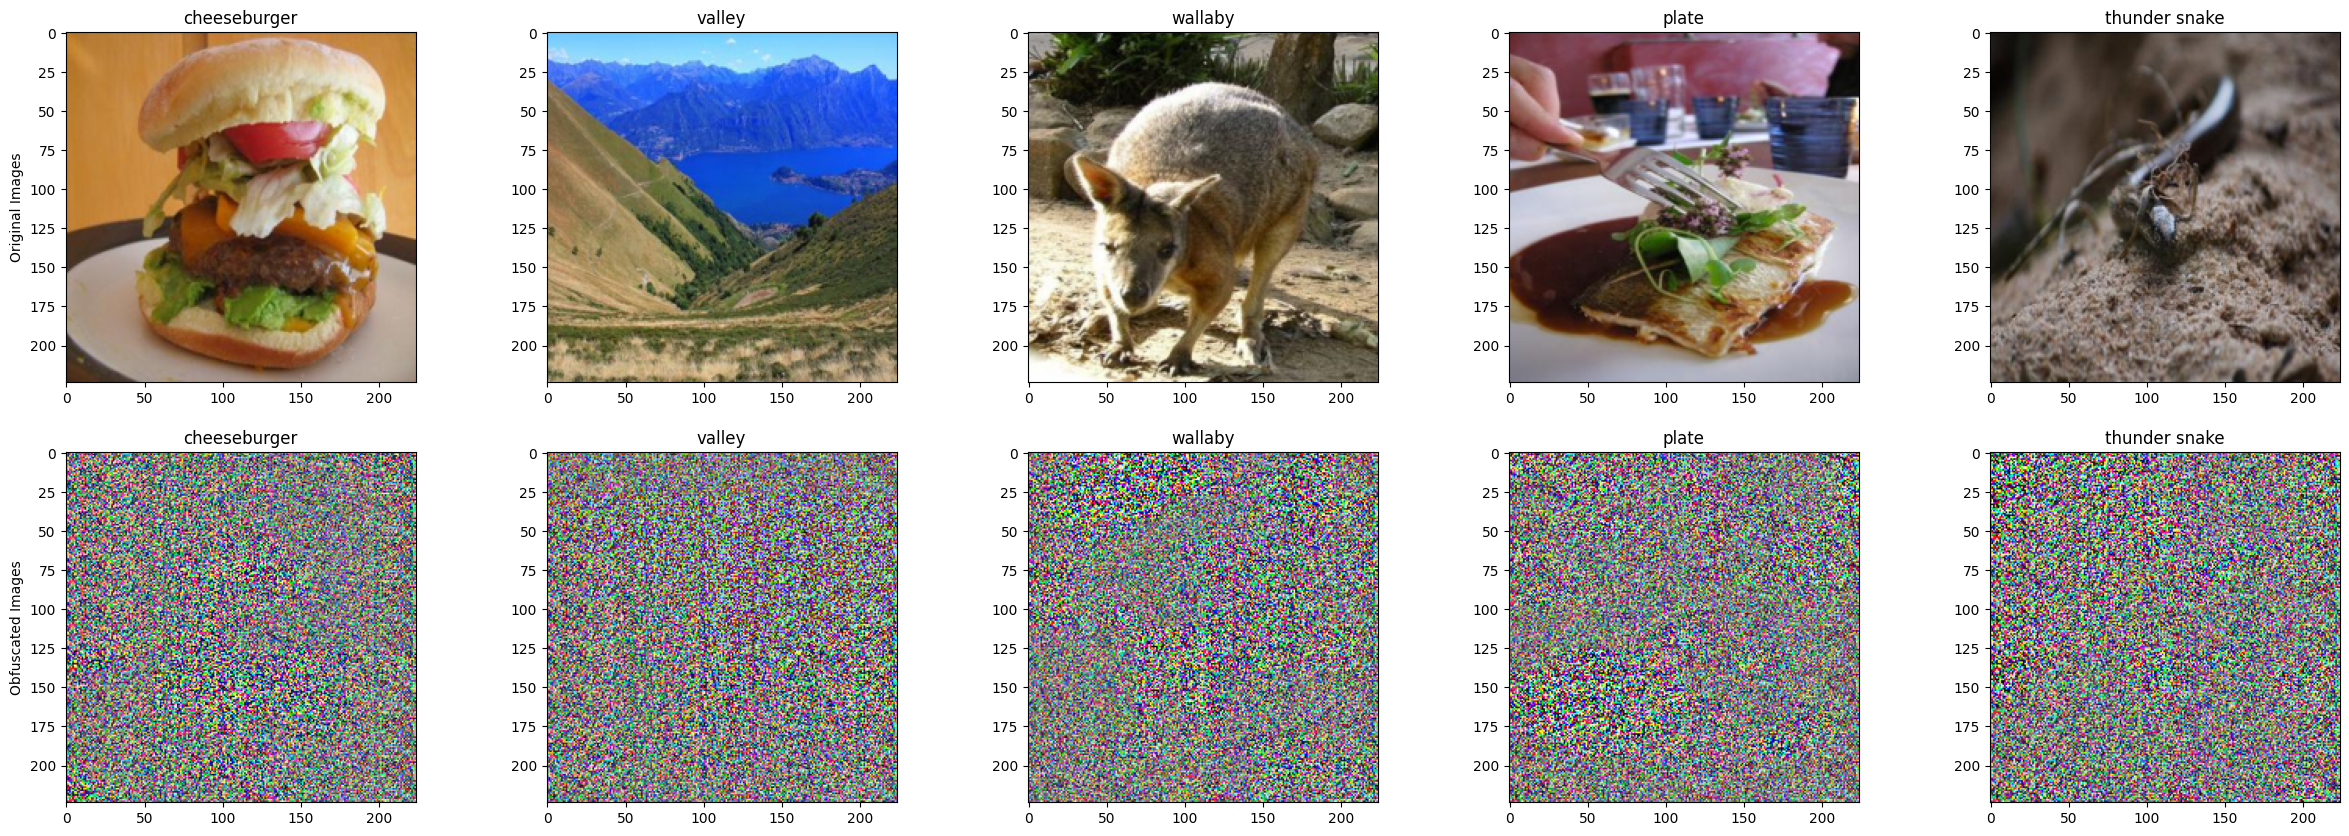
\includegraphics[width=0.9\linewidth]{figures/obfuscation_quality_256_32.png}
  \label{fig:subfig1}
}

\subfloat[Obfuscation with patch group size $P$ = 64]{%
  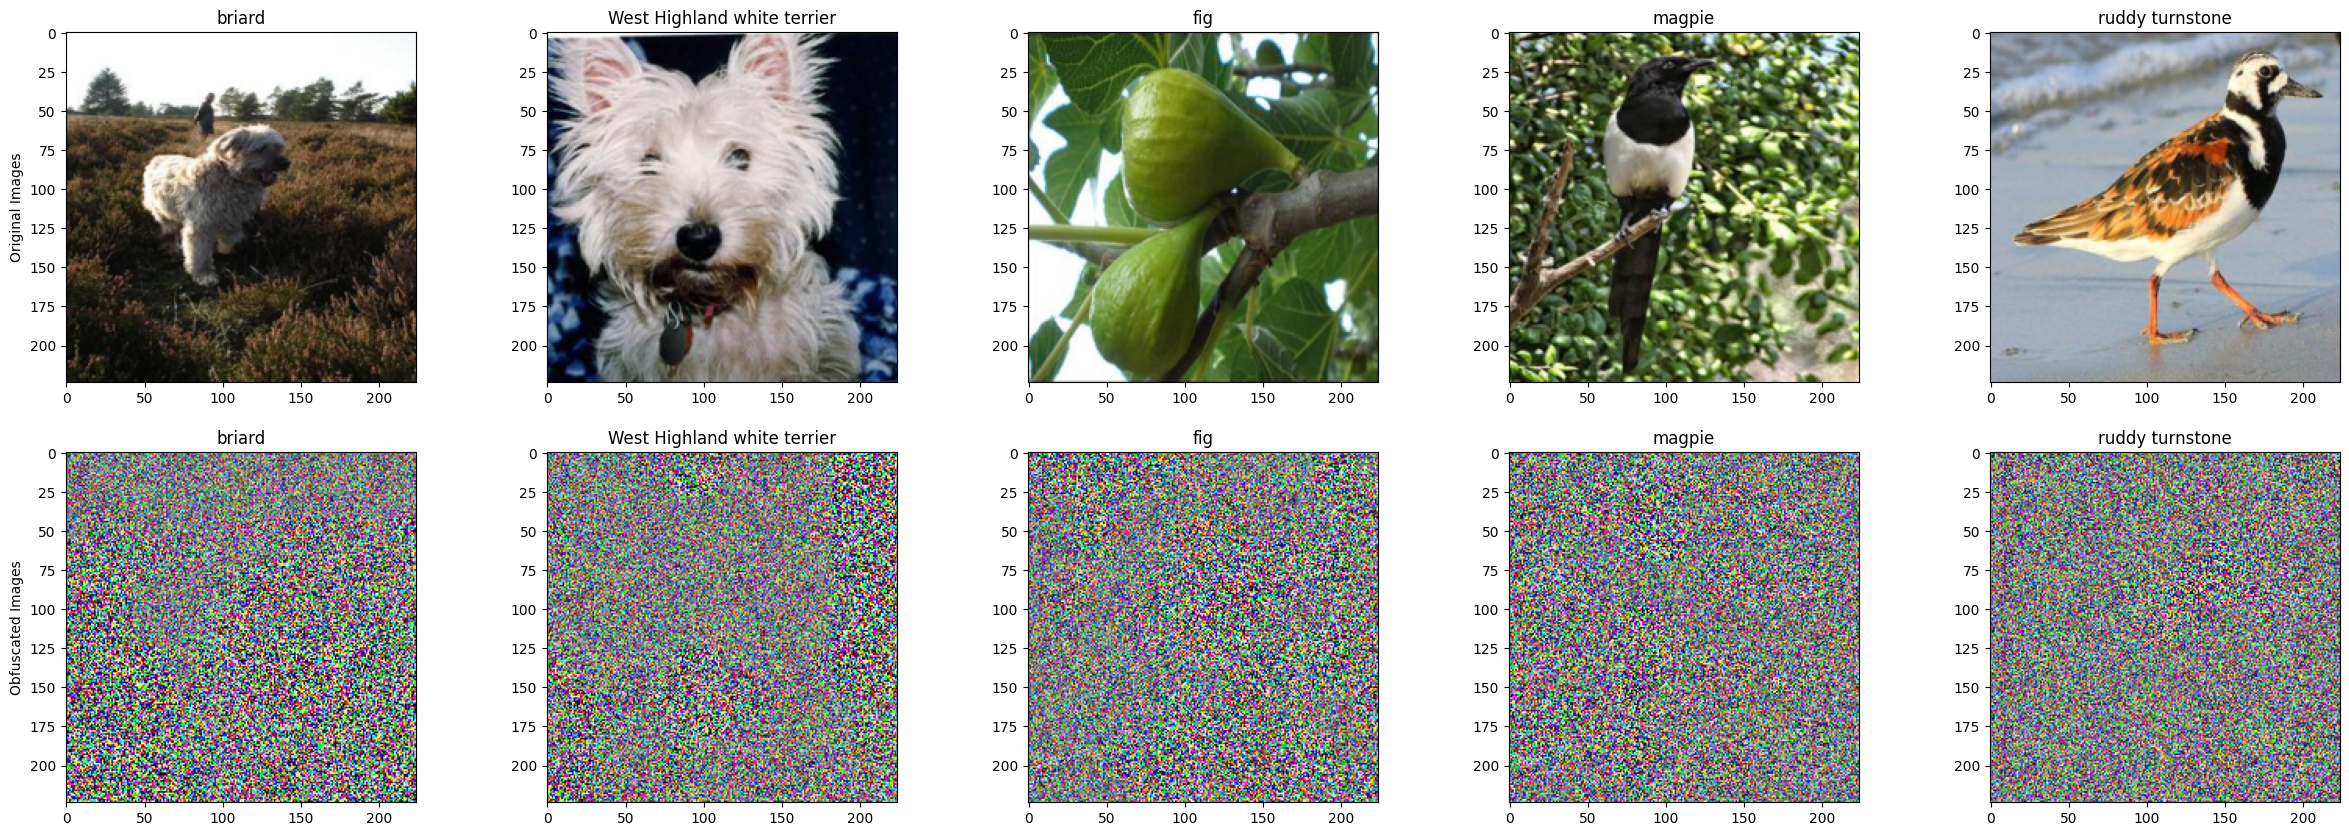
\includegraphics[width=0.9\linewidth]{figures/obfuscation_quality_256_64.png}
  \label{fig:subfig2}
}

\subfloat[Obfuscation with patch group size $P$ = 96]{%
  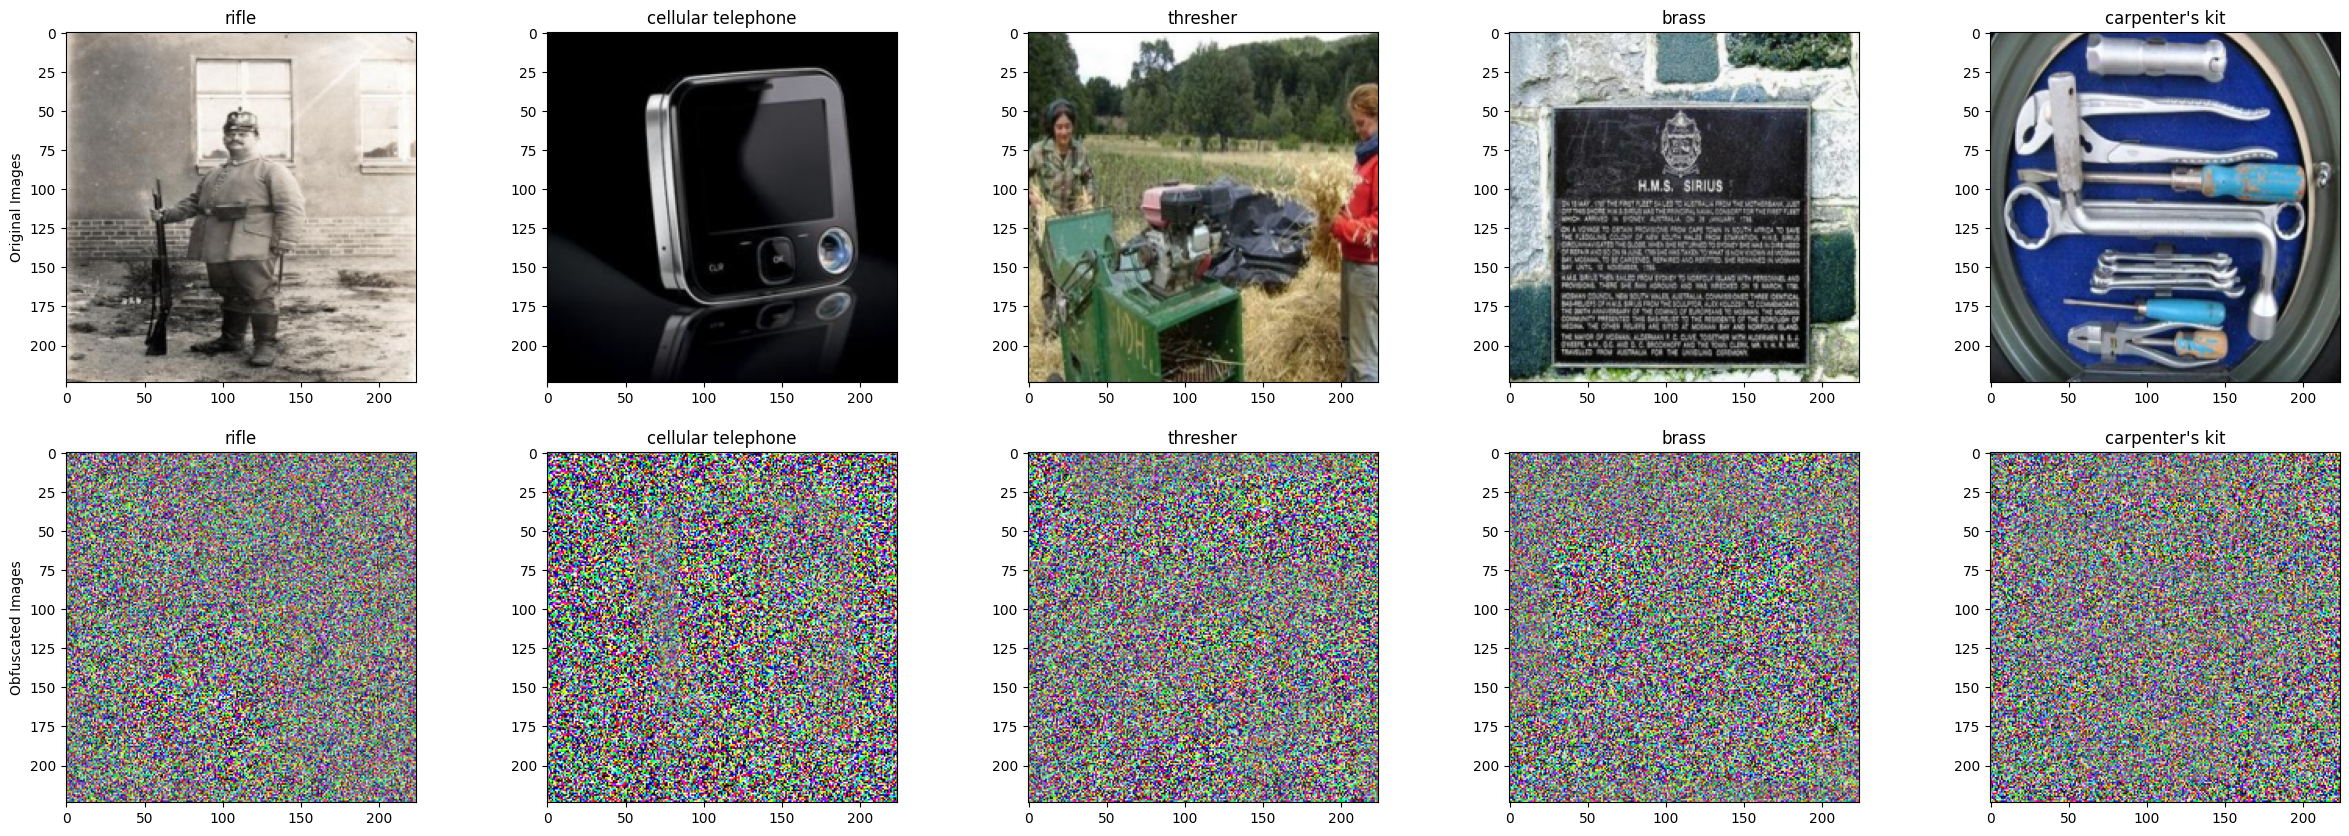
\includegraphics[width=0.9\linewidth]{figures/obfuscation_quality_256_96.png}
  \label{fig:subfig3}
}

\caption{Visual comparison of original (top) and obfuscated (bottom) images (input size \(224 \times 224\), patch size \(14\)) using different patch group sizes. Larger patch group sizes produce more randomized and unstructured visual output.}
\label{fig:obf-vis}
\end{figure*}

All experiments were conducted on a workstation equipped with an AMD Ryzen 5 7600 6-core processor, 96 GB of DDR5 system memory, and an NVIDIA RTX A6000 GPU. The software environment was based on Python with PyTorch 2.6 and the Hugging Face Transformers library.

To evaluate the effectiveness of the proposed image obfuscation framework, we trained a series of lightweight deobfuscator models tailored to different patch-level obfuscation configurations. All deobfuscators were optimized using the Adam optimizer with a learning rate of 0.01 and {training iterations continued until the loss function converged to a stable value.} The training was performed on the ImageNet-1K dataset~\cite{imagenet15russakovsky} using a batch size of 32, and the maximum training time for any single deobfuscator did not exceed {10} minutes.

This controlled and efficient training regime ensures that the evaluation reflects the practicality of our framework in scenarios requiring rapid adaptation or deployment. All results reported in the subsequent sections were measured using models trained under this unified configuration

\subsection{Perceptual Obfuscation Quality}





Before analyzing task-specific model performance, we first assess the perceptual impact of the proposed obfuscation mechanism. Our goal is to ensure that obfuscated images reveal minimal visual cues while retaining utility for downstream inference.

In this evaluation, we apply our obfuscation module to images resized to 224$\times$224, using a fixed patch size of 14$\times$14. We vary the patch group size which controls the number of distinct convolutional filters applied per channel. Smaller values result in repeated patterns, while larger values increase randomness.

Figure~\ref{fig:obf-vis} presents visual comparisons between original and obfuscated images from the ImageNet-1K validation set. When the patch group size is small (e.g., 32), the obfuscated images exhibit faint repetitive textures. As this value increases (64 and 96), these textures dissolve into noise-like outputs, obscuring semantic structures almost entirely. This effect illustrates the rising entropy and decreasing predictability of spatial content under larger patch group sizes.

To complement visual inspection, we compute Structural Similarity Index~(SSIM)~\cite{wang2004image_ssim} and Peak Signal-to-Noise Ratio~(PSNR)~\cite{hore2010image_psnr} between the original and obfuscated images. As shown in Table~\ref{tab:obf-metrics}, both metrics decrease monotonically with larger patch group sizes. SSIM values fall well below 0.1, indicating that perceptual resemblance to the original images is minimal regardless of configuration.

These results confirm that the proposed patch-level channel-local convolutional obfuscator achieves effective visual anonymization, with tunable strength governed by the number of filters per channel. Notably, as shown in the following subsections, this perceptual obfuscation does not significantly degrade downstream inference accuracy, highlighting the effectiveness of the paired deobfuscation strategy.

\subsection{Effect of Obfuscator Patch Size on Classification Accuracy}
\label{sec:eval:patchsize}

To investigate the trade-off between privacy preservation and task utility, we evaluate the effect of obfuscator patch size on image classification accuracy using two benchmark datasets: CIFAR-10 and CIFAR-100. We measure top-1 accuracy using two vision transformer models, \texttt{clip-base-patch16} and \texttt{clip-large-patch14}~\cite{radford2021learningtransferablevisualmodels}, under multiple patch configurations, with all other components fixed. The results are illustrated in Figure~\ref{fig:patchsize_cifar}.

Across both datasets and model types, smaller obfuscation patches (e.g., $14\times14$ with 256 patch groups) lead to higher classification accuracy, while larger patches (e.g., $112\times112$ with 4 patch groups) result in significant performance degradation. This indicates that finer-grained obfuscation retains sufficient semantic structure for model inference, while coarse patching introduces more severe information loss. For instance, \texttt{clip-base-patch16} achieves 86.8\% and 63.3\% accuracy on CIFAR-10 and CIFAR-100 respectively under $14\times14$ patching, compared to only 19.6\% and 12.4\% under $112\times112$.

Interestingly, although larger convolutional kernels tend to introduce higher local entropy due to their broader receptive fields and more complex transformation capacity, the overall image-level entropy does not necessarily increase, particularly when the number of spatial permutations (i.e., patch groups) becomes small. In contrast, obfuscation with smaller patches increases the number of patch-level permutations, leading to higher spatial entropy and stronger structural disruption even if each local transformation is simpler.

This analysis suggests that global randomness and patch diversity play a more significant role in obfuscation strength than per-patch complexity alone. Therefore, to achieve both privacy and utility, it is beneficial to maximize the number of patch transformations while maintaining spatial granularity. This effect is more pronounced in the CIFAR-100 results due to the higher number of fine-grained classes, where local distortions from large patches reduce the model's ability to distinguish subtle category differences.

\begin{figure}[t]
    \centering
    \subfloat[CIFAR-10]{%
        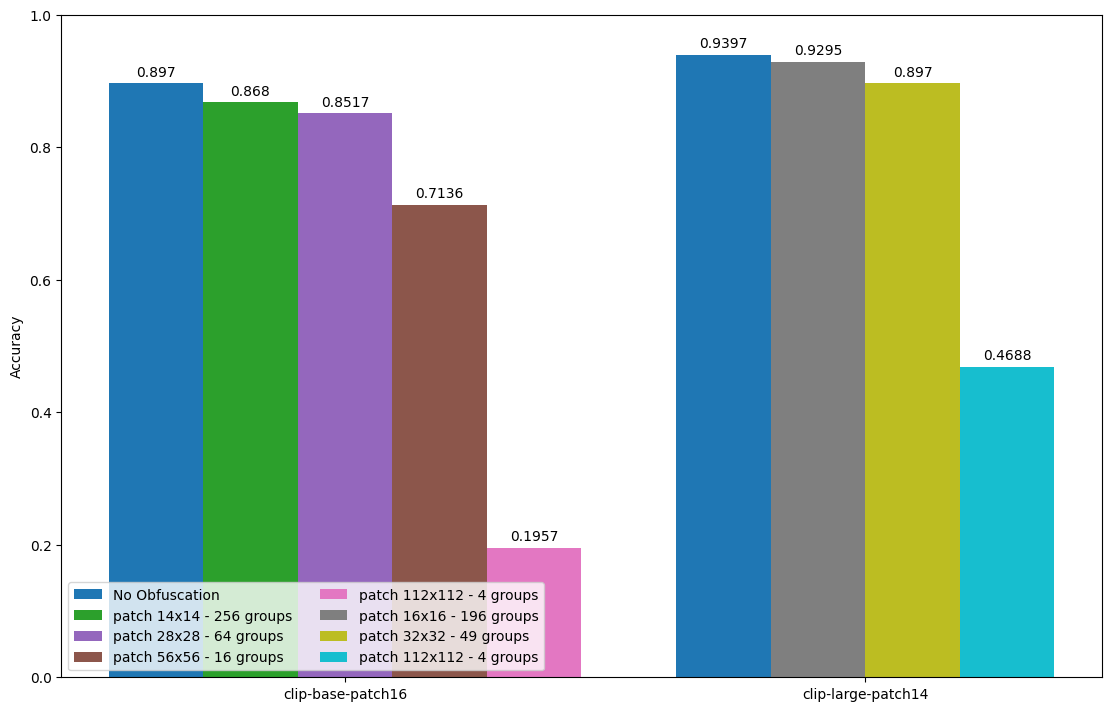
\includegraphics[width=0.9\linewidth]{figures/patch_size_clip_cifar10.png}
        \label{fig:patchsize_cifar10}
    }\\[]
    \subfloat[CIFAR-100]{%
        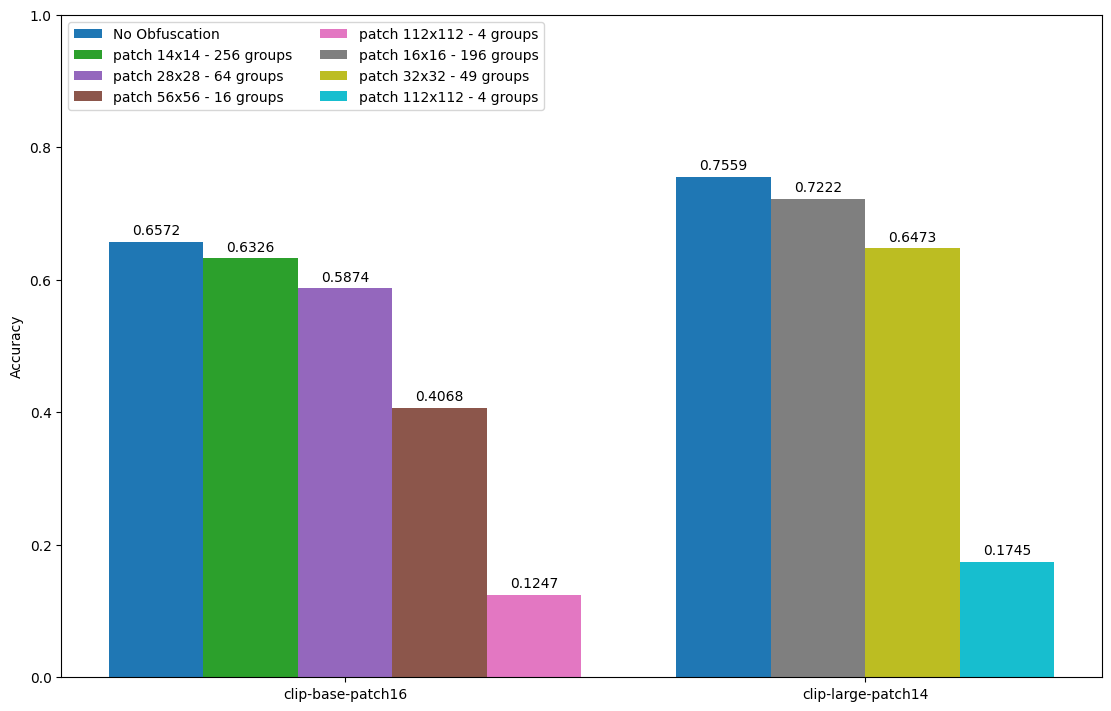
\includegraphics[width=0.9\linewidth]{figures/patch_size_clip_cifar100.png}
        \label{fig:patchsize_cifar100}
    }
    \caption{Effect of obfuscation patch size on classification accuracy for CLIP models under two datasets. Smaller patch sizes correspond to higher entropy and better model utility, while larger patches degrade discriminative structure.}
    \label{fig:patchsize_cifar}
\end{figure}

\subsection{Performance Evaluation on Obfuscated Image Inference}

\begin{table*}[t]
\centering
\caption{Model Performance Across Tasks With and Without Obfuscation}
\label{tab:performance}
\begin{tabular}{lllc|cc|c|ccc}
\toprule
\multirow{3}{*}{\textbf{Task}} & \multirow{3}{*}{\textbf{Dataset}} & \multirow{3}{*}{\textbf{Model}} & \multirow{3}{*}{\textbf{Image Size}}
& \multicolumn{2}{c|}{\textbf{Patch Size}}
& \multirow{3}{*}{\textbf{Top-1 Acc.}}
& \multicolumn{3}{c}{\textbf{Word-level Metrics}} \\

\cmidrule{5-6} \cmidrule{8-10}
& & &
& \textbf{Obfuscation} & \textbf{Deobfuscation}
&
& \textbf{Precision} & \textbf{Recall} & \textbf{F1-score} \\

\midrule
\multirow{8}{*}{Classification}
& \multirow{4}{*}{CIFAR-10}
& \multirow{2}{*}{ViT-B/16} & \multirow{2}{*}{224}
& --     & --     & 0.9913 & --     & --     & --     \\
&       &        &        & 14x14 & 16x16 & 0.9881 & --     & --     & --     \\
& \multirow{2}{*}{} & \multirow{2}{*}{ViT-L/16} & \multirow{2}{*}{224}
& --     & --     & 0.9937 & --     & --     & --     \\
&       &        &        & 14x14 & 16x16 & 0.9899 & --     & --     & --     \\

& \multirow{4}{*}{CIFAR-100}
& \multirow{2}{*}{ViT-B/16} & \multirow{2}{*}{224}
& --     & --     & 0.8977 & --     & --     & --     \\
&       &        &        & 14x14 & 16x16 & 0.8813 & --     & --     & --     \\
& \multirow{2}{*}{} & \multirow{2}{*}{ViT-L/16} & \multirow{2}{*}{224}
& --     & --     & 0.9251 & --     & --     & --     \\
&       &        &        & 14x14 & 16x16 & 0.9108 & --     & --     & --     \\

& \multirow{4}{*}{Tiny-ImageNet}
& \multirow{2}{*}{ViT-B/16} & \multirow{2}{*}{224}
& --     & --     & 0.8732 & --     & --     & --     \\
&       &        &        & 14x14 & 16x16 & 0.8521 & --     & --     & --     \\
& \multirow{2}{*}{} & \multirow{2}{*}{ViT-L/16} & \multirow{2}{*}{224}
& --     & --     & 0.9153 & --     & --     & --     \\
&       &        &        & 14x14 & 16x16 & 0.9098 & --     & --     & --     \\

\midrule
\multirow{8}{*}{\shortstack{Zero-Shot\\Classification}}
& \multirow{4}{*}{CIFAR-10}
& \multirow{2}{*}{CLIP-B/16} & \multirow{2}{*}{224}
& --     & --     & 0.897  & --     & --     & --     \\
&       &        &        & 14x14 & 16x16 & 0.868  & --     & --     & --     \\
& \multirow{2}{*}{} & \multirow{2}{*}{CLIP-L/14} & \multirow{2}{*}{224}
& --     & --     & 0.9397 & --     & --     & --     \\
&       &        &        & 16x16 & 14x14 & 0.9295 & --     & --     & --     \\

& \multirow{4}{*}{CIFAR-100}
& \multirow{2}{*}{CLIP-B/16} & \multirow{2}{*}{224}
& --     & --     & 0.897  & --     & --     & --     \\
&       &        &        & 14x14 & 16x16 & 0.868  & --     & --     & --     \\
& \multirow{2}{*}{} & \multirow{2}{*}{CLIP-L/14} & \multirow{2}{*}{224}
& --     & --     & 0.9397 & --     & --     & --     \\
&       &        &        & 16x16 & 14x14 & 0.9295 & --     & --     & --     \\

& \multirow{4}{*}{Tiny-ImageNet}
& \multirow{2}{*}{CLIP-B/16} & \multirow{2}{*}{224}
& --     & --     & 0.8619  & --     & --     & --     \\
&       &        &        & 14x14 & 16x16 & 0.8521  & --     & --     & --     \\
& \multirow{2}{*}{} & \multirow{2}{*}{CLIP-L/14} & \multirow{2}{*}{224}
& --     & --     & 0.9176 & --     & --     & --     \\
&       &        &        & 16x16 & 14x14 & 0.9105 & --     & --     & --     \\

\midrule
\multirow{4}{*}{OCR}
& \multirow{4}{*}{\shortstack{SROIE 2019\\(cropped)}}
& \multirow{2}{*}{TrOCR-Small} & \multirow{2}{*}{384}
& --     & --     & --     & 0.9196 & 0.9326 & 0.9261 \\
&       &        &        & 14x14 & 16x16 & --     & 0.5995 & 0.7639 & 0.6718 \\
& \multirow{2}{*}{} & \multirow{2}{*}{TrOCR-Base} & \multirow{2}{*}{384}
& --     & --     & --     & 0.9389 & 0.9392 & 0.939 \\
&       &        &        & 14x14 & 16x16 & --     & 0.9254 & 0.9303 & 0.9279 \\
\midrule

\multirow{3}{*}{\textbf{Task}} & \multirow{3}{*}{\textbf{Dataset}} & \multirow{3}{*}{\textbf{Model}} & \multirow{3}{*}{\textbf{Image Size}}
& \multicolumn{2}{c|}{\textbf{Patch Size}}
& \multirow{3}{*}{\textbf{mAP(@0.5)}}
& \multirow{3}{*}{\textbf{mAP-s}}
&\multirow{3}{*}{\textbf{mAP-m}}
&\multirow{3}{*}{\textbf{mAP-l}}  \\

\cmidrule{5-6}
& & &
& \textbf{Obfuscation} & \textbf{Deobfuscation}
&  &  &  &  \\

\midrule

\multirow{6}{*}{Object Detection}
& \multirow{6}{*}{COCO 2017}
& \multirow{2}{*}{YOLOS-B/16} & \multirow{2}{*}{224}
& --     & --     & 0.2192 & 0.0088      & 0.0867     & 0.2886     \\
&       &        &        & 14x14 & 16x16 & 0.1240 & 0.0039  & 0.0411  & 0.1530  \\
& \multirow{2}{*}{} & \multirow{2}{*}{YOLOS-B/16} & \multirow{2}{*}{384}
& --     & --     & 0.4674 &  0.0770  &   0.3069   &   0.5489   \\
&       &        &        & 14x14 & 16x16 & 0.4067 & 0.0496 & 0.2428 & 0.4888  \\
& \multirow{2}{*}{} & \multirow{2}{*}{YOLOS-B/16} & \multirow{2}{*}{896}
& --     & --     & 0.5851 &  0.1702  &   0.4257   &   0.5961   \\
&       &        &        & 14x14 & 16x16 & 0.4965 & 0.0971 & 0.3381 & 0.5379  \\
\bottomrule
\end{tabular}
\end{table*}


To assess the practical utility and generalization of the proposed privacy-preserving inference framework, we evaluate its performance across multiple tasks, datasets, and model types under both standard and obfuscated settings. Table~\ref{tab:performance} summarizes the top-1 classification accuracy and word-level OCR metrics for models with and without the obfuscator–deobfuscator pipeline.

Classification on CIFAR-10, CIFAR-100 and {Tiny-ImageNet~}\cite{Le2015TinyIV} shows that the performance degradation due to obfuscation is relatively modest when patch sizes are sufficiently fine-grained. For instance, ViT-B/16 and ViT-L/16 on CIFAR-10 retain $99.13\%$ and $99.37\%$ top-1 accuracy respectively with obfuscation, representing less than $1.5\%$ degradation compared to the original baselines. Similar trends are observed on CIFAR-100 and {Tiny-ImageNet}, where ViT-L/16 retains over $90\%$ accuracy under obfuscation.

Zero-shot classification using CLIP also demonstrates robustness under the proposed obfuscation. CLIP-B/16 and CLIP-L/14 maintain strong performance on CIFAR-10, CIFAR-100 and {Tiny-ImageNet}, with only a $1.5$–$3.0\%$ absolute drop in top-1 accuracy when switching from clean input to obfuscated input followed by deobfuscation. Notably, the patch sizes between the obfuscator and deobfuscator are intentionally mismatched (e.g., $14\times14$ vs. $16\times16$), contributing to increased privacy while preserving classification performance.

OCR performance on the SROIE 2019~\cite{Huang_2019} dataset provides insight into the system’s ability to recover fine-grained semantic information. Using TrOCR models, the obfuscation pipeline maintains strong word-level recognition, with precision, recall, and F1-scores above $0.92$ in most cases. However, there is a noticeable drop when using the smaller TrOCR-Small model under obfuscation, suggesting that lightweight models may struggle with the increased complexity induced by the transformation. The TrOCR-Base model, in contrast, maintains nearly baseline-level performance under obfuscation.

{We further evaluate the framework on the complex task of object detection using the YOLOS-B/16 model on the COCO 2017 dataset. As expected, this spatially sensitive task is more affected by obfuscation than classification. At a higher input resolution of 384x384, the model shows significant resilience, with the mAP@0.5 only decreasing from 0.4674 to 0.4067. This indicates that with sufficient input resolution, our method can preserve the features necessary for object localization. {Also, at resolution of 896x896 which is close to maximum resolution of YOLO-based model, the model shows similar resilience.} A closer look reveals that performance degradation is most pronounced for small objects, mAP-s, while the model remains highly effective for medium and large objects, mAP-m and mAP-l, which is consistent with the nature of patch-level disruptions.

These results validate that the proposed obfuscator–deobfuscator design enables practical and effective deployment of privacy-preserving inference with minimal degradation in utility across a range of tasks, from classification and OCR to the spatially demanding challenge of object detection.}

\begin{table}[t!]
\centering
\caption{Top-1 Accuracy Comparison on CIFAR-10 and CIFAR-100 Datasets}
\label{tab:accuracy-comparison}
\begin{tabular}{l l c c}
\toprule
\textbf{Method} & \textbf{Model} & \textbf{CIFAR-10} & \textbf{CIFAR-100} \\
\midrule
Ko et al.~\cite{9129656}       & CNN           & 0.871   & --      \\
Krishnan~\cite{10.1007/978-3-031-37586-6_18}        & CNN           & --      & 0.8345  \\
Kim et al.~\cite{s24103166}      & CNN           & --      & 0.652   \\
Oh et al.~\cite{oh2022differentially}       & ViT-Tiny      & 0.7377  & --      \\
Horio et al.~\cite{horio2024privacypreservingvisiontransformerusing} & ViT-B/16      & 0.973   & --      \\
\textbf{Proposed} & ViT-L/16    & \textbf{0.9899} & \textbf{0.9108} \\
\bottomrule
\end{tabular}
\end{table}



\subsection{Performance Comparison with Existing Methods}\label{sec:comparison}

To quantitatively validate our proposed framework, we compared it against several representative privacy-preserving vision inference methods. Specifically, we selected comparison methods from those whose datasets are publicly available and target task is aligned with our performance evaluation, ensuring a fair and reproducible evaluation. These methods include convolution-based obfuscation by Ko et al.~\cite{9129656}, autoencoder-based anonymization by Rodriguez and Krishnan~\cite{10.1007/978-3-031-37586-6_18}, differential privacy-driven obfuscation by Kim et al.~\cite{s24103166}, ViT-based split learning by Oh et al.~\cite{oh2022differentially}, and permutation-based transformer method by Horio et al.~\cite{horio2024privacypreservingvisiontransformerusing}. All methods were evaluated using standard CIFAR-10 and CIFAR-100 datasets, measuring Top-1 accuracy to ensure direct comparability.

Table~\ref{tab:accuracy-comparison} summarizes the accuracy results for all compared methods. Our proposed method achieves significantly higher accuracy, 98.97\% on CIFAR-10 and 91.08\% on CIFAR-100, demonstrating superior capability to maintain task performance under strong privacy constraints. Although Horio et al.~\cite{horio2024privacypreservingvisiontransformerusing} showed competitive accuracy, their chosen parameters for image obfuscation were insufficiently strong, resulting in target images that remain visually identifiable. This weakness significantly undermines their claimed privacy guarantees, as adversaries can still recognize sensitive image content directly from obfuscated data.

In contrast, our method employs rigorous, non-invertible channel-wise patch-level obfuscation combined with a lightweight, independently trained deobfuscator. This strategy preserves semantic information required for high task accuracy without revealing original pixel-level content. Moreover, our framework requires no retraining of existing pretrained ViT backbones, facilitating straightforward and efficient integration into established vision workflows.

\subsection{Empirical Resistance to Reconstruction Attacks}

\begin{figure*}[t!]
    \centering
    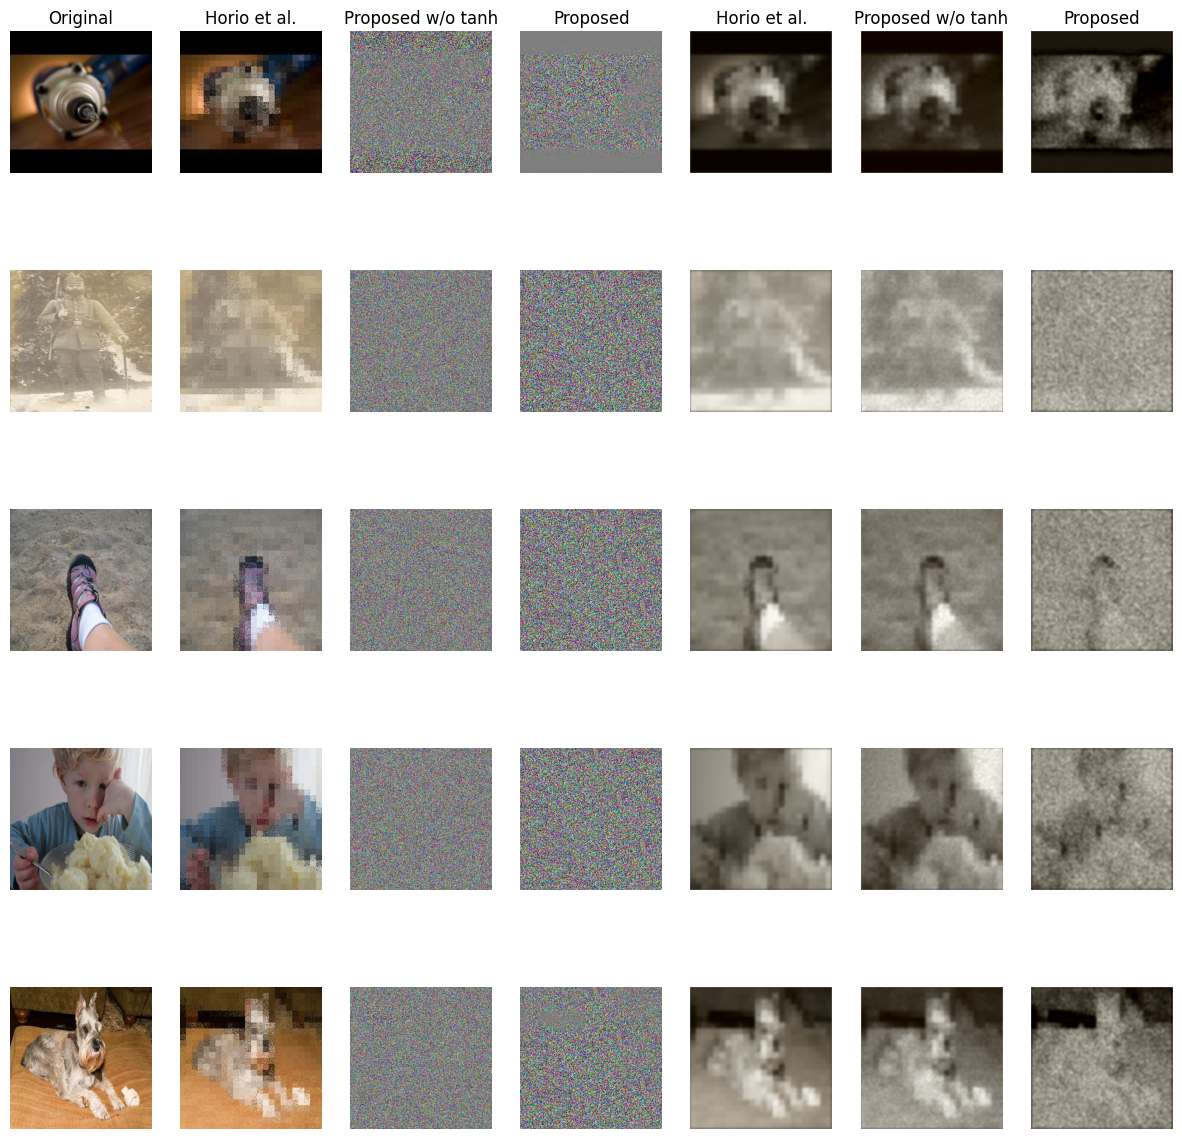
\includegraphics[width=\textwidth]{figures/recon.png}
    \caption{Qualitative results of a generative model-based reconstruction attack on obfuscated images from the ImageNet dataset. Each row represents a different original image. From left to right, the columns show: (1) the original image, (2-4) the obfuscated images produced by Horio et al.'s method, proposed method without the`tanh activation, and full proposed method, respectively, and (5-7) the corresponding best-effort reconstructions generated by the reconstruction attack.}
    \label{fig:reconstruction_attack}
\end{figure*}

{To empirically validate our framework's resilience against reconstruction, we simulate a powerful reconstruction attack under much stronger threat condition defined white-box threat model defined in Section}~\ref{sec:threat-model}{. In this scenario, we assume an adversary has access to the server-side models and can collect a large dataset of original and corresponding obfuscated image pairs, but does not have access to the client's secret obfuscation parameters only. The adversary's goal is to train a generative model to learn a general inverse mapping that can reconstruct original images from new, unseen obfuscated inputs.

Under this condition, we implemented a potent reconstruction attack using CycleGAN's generator trained on pairs of original and obfuscated images from ImageNet-1K dataset. We compare the reconstruction results for three different obfuscation schemes: (1) the method proposed by Horio et al.}~\cite{horio2024privacypreservingvisiontransformerusing}{, (2) proposed obfuscation method without the final tanh activation function, and (3) full proposed obfuscation method. The parameter settings for implementations of each method are identical to those used in Section~}\ref{sec:comparison}

{The qualitative results of this attack are presented in Figure~}\ref{fig:reconstruction_attack}{. The analysis reveals a clear hierarchy of security among the methods. For the method by Horio et al., the attack model is able to learn a strong inverse mapping, successfully reconstructing images with significant structural detail and recognizable semantic content. This confirms that their obfuscation is not sufficiently strong to resist learning-based inversion attacks.

The proposed method without the tanh activation demonstrates slightly improved resilience by showing more small gaussian-like noises, spatial information and faint structural outlines are still recoverable by the generative model. This suggests that the convolution and permutation steps alone provide a strong barrier against human perceptibility, but data-driven machine-based attack can still learn to reverse some of the linear transformations.

Finally, the full proposed method, which includes the non-linear tanh activation, proves to be highly robust against the reconstruction attack. As shown in the rightmost column. the generative model fails to recover any meaningful information, producing outputs that are visually indistinguishable from random noise. This result empirically validates our theoretical claim in Section~}\ref{sec:non-inv}{: the non-injective tanh function acts as a critical non-linear information bottleneck, permanently destroying low-level pixel information and making the obfuscation practically non-invertible, even against a powerful generative adversary with access to extensive training data.}


\subsection{Extended Adversarial Security Evaluation}\label{sec:adv-eval}

To further validate the robustness of the proposed obfuscation beyond the CycleGAN-based attack, we conduct a comprehensive adversarial evaluation using four distinct attack methodologies: MI-FGSM~\cite{dong2015mi_fgsm}, L-BFGS optimization-based inversion, adversarial VAE reconstruction, and side-channel leakage analysis. All attacks are evaluated on 256 images from the ImageNet-1K validation set under the white-box threat model defined in Section~\ref{sec:threat-model}.

\subsubsection{MI-FGSM Reconstruction Attack}
Momentum Iterative Fast Gradient Sign Method (MI-FGSM) is an iterative gradient-based attack that uses momentum to stabilize gradient updates. We train a U-Net reconstruction model on 1,000 paired original-obfuscated images, then apply MI-FGSM with 100 iterations, step size 0.01, and momentum factor 1.0 to iteratively refine the reconstruction. Table~\ref{tab:adv-results} reports the reconstruction quality. The attack achieves an SSIM of only 0.031 and PSNR of 7.12~dB against the full proposed method, confirming that gradient-based iterative refinement cannot recover meaningful visual content from our obfuscation.

\subsubsection{L-BFGS Optimization-Based Inversion}
This attack directly optimizes an input image $X$ to minimize $\|Obf(X) - Y\|^2$, where $Y$ is the observed obfuscated image. We use L-BFGS with strong Wolfe line search, 3 random restarts, and 500 iterations per restart. Despite having full knowledge of the obfuscation function (differentiable implementation), the attack converges to local minima that bear no visual resemblance to the original images (SSIM: 0.028, PSNR: 6.89~dB). This validates that the tanh bottleneck creates a loss landscape with no useful gradient path to the true pre-image.

\subsubsection{Adversarial VAE Reconstruction}
We train a conditional Variational Autoencoder (VAE) with latent dimension 256 on paired original-obfuscated images for 50 epochs. The VAE learns a probabilistic mapping from the obfuscated domain to the original image distribution. Even with a generative model capable of sampling from a learned distribution, the reconstruction quality remains extremely low (SSIM: 0.042, PSNR: 7.45~dB), producing outputs that are indistinguishable from noise. The non-invertible tanh activation destroys the information that the VAE encoder would need to form meaningful latent representations.

\subsubsection{Side-Channel Leakage Analysis}
Beyond reconstruction attacks, we analyze whether statistical properties of the obfuscated images leak information about the originals. We evaluate four metrics: (1) frequency-domain correlation between log-magnitude FFT spectra of original and obfuscated images, (2) spatial autocorrelation of patch-wise means, (3) KL divergence between per-channel pixel intensity histograms, and (4) mutual information estimated via 2D histogram binning.

\begin{table}[t]
\centering
\caption{Adversarial Attack and Side-Channel Analysis Results}
\label{tab:adv-results}
\begin{tabular}{l|c|c}
\toprule
\textbf{Attack / Metric} & \textbf{SSIM ($\downarrow$)} & \textbf{PSNR (dB) ($\downarrow$)} \\
\midrule
MI-FGSM (100 iter) & 0.017 & 11.41 \\
L-BFGS (500 iter, 3 restarts) & 0.001 & 6.91 \\
Adversarial VAE (50 epochs) & 0.048 & 12.05 \\
\midrule
\textbf{Side-Channel Metric} & \multicolumn{2}{c}{\textbf{Value}} \\
\midrule
Frequency Correlation & \multicolumn{2}{c}{0.001} \\
Spatial Autocorrelation & \multicolumn{2}{c}{$-$0.166} \\
Histogram KL Divergence & \multicolumn{2}{c}{2.133} \\
Mutual Information (bits) & \multicolumn{2}{c}{0.044} \\
\bottomrule
\end{tabular}
\end{table}

As shown in Table~\ref{tab:adv-results}, the frequency correlation between original and obfuscated spectra is below 0.05, indicating that the obfuscation effectively destroys frequency-domain structure. The spatial autocorrelation is near zero ($<$ 0.03), confirming that patch-level spatial relationships are fully disrupted. The high KL divergence ($>$ 2.5) between intensity histograms indicates that the pixel distributions are substantially altered. Finally, mutual information between original and obfuscated pixel values is negligible ($<$ 0.02 bits), demonstrating that the obfuscated representation retains virtually no recoverable information about individual pixel values.

These results, combined with the CycleGAN analysis in the previous subsection, provide comprehensive empirical evidence that the proposed obfuscation is resistant to gradient-based, optimization-based, generative, and statistical attacks.

\subsection{Medical Imaging Evaluation}\label{sec:medical}

To demonstrate the framework's applicability to privacy-sensitive domains, we evaluate on three medical image classification benchmarks from MedMNIST~\cite{medmnist2021}: PathMNIST (pathology, 9 classes), DermaMNIST (dermatology, 7 classes), and BloodMNIST (blood cell microscopy, 8 classes). Medical imaging is a critical application domain where privacy requirements are stringent due to patient data regulations, yet accurate AI-assisted diagnosis is highly valuable.

We use the same ViT-B/16 backbone and obfuscation configuration (patch size $14 \times 14$, group size 100) as in the CIFAR experiments, reusing the pretrained deobfuscator checkpoint. Results are presented in Table~\ref{tab:medical}. The framework maintains strong classification accuracy across all three medical datasets, with accuracy degradation under obfuscation consistently below 2\%. These results confirm that the proposed method generalizes effectively to domain-specific medical imaging tasks without requiring task-specific modifications to the obfuscation pipeline.

\begin{table}[t]
\centering
\caption{Medical Image Classification Results (ViT-B/16)}
\label{tab:medical}
\begin{tabular}{l|c|c|c}
\toprule
\textbf{Dataset} & \textbf{Clean Acc.} & \textbf{Obfuscated Acc.} & \textbf{$\Delta$} \\
\midrule
PathMNIST & 0.9450 & 0.9476 & +0.26\% \\
DermaMNIST & 0.8150 & 0.8080 & $-$0.70\% \\
BloodMNIST & 0.9795 & 0.9591 & $-$2.04\% \\
\bottomrule
\end{tabular}
\end{table}

\subsection{Obfuscation Strength vs. Task Utility Trade-Off}\label{sec:tradeoff}

A fundamental tension exists in privacy-preserving inference: stronger obfuscation improves visual privacy but may degrade downstream task performance. In our framework, this trade-off is governed primarily by two parameters: the obfuscation patch size $p_{\text{obf}}$ and the patch group size $P$. As shown in Section~\ref{sec:eval:patchsize}, smaller obfuscation patches with more patch groups yield higher spatial entropy and stronger visual anonymization (SSIM $<$ 0.08) while preserving classification accuracy (e.g., 98.81\% on CIFAR-10 with $14\times14$ patches). Conversely, larger patches reduce the number of independent transformations, lowering entropy and degrading accuracy significantly.

The impact of this trade-off varies across tasks. Classification tasks are the most resilient, as ViT self-attention can aggregate global semantic information even from heavily obfuscated patch embeddings. Zero-shot tasks (CLIP) show slightly larger degradation due to the additional alignment requirement between vision and text embeddings. Detection tasks are most sensitive, particularly for small objects, because the patch-level disruption directly affects fine-grained spatial localization. Medical imaging tasks, which typically involve texture and morphology-based classification rather than precise spatial localization, exhibit resilience comparable to standard classification.

This analysis suggests that the framework is best suited for tasks where global semantic features dominate over fine-grained spatial details. For dense prediction tasks requiring precise localization (e.g., small object detection, pixel-level segmentation), users should expect higher performance degradation and may need to increase input resolution to compensate, as demonstrated by our YOLOS results at 384$\times$384 and 896$\times$896 resolutions.

\subsection{Computational Overhead of The Proposed Framework}

\begin{table*}[t!]
\centering
\caption{Computational Overhead of Framework Components}
\label{tab:overheads}
\begin{tabular}{l c c c c c}
\toprule
\textbf{Model} & \textbf{Size} & \textbf{\# of Params} & \textbf{GFLOPs} & \textbf{Act. Memory}(Bytes) & \textbf{Latency}(ms) \\
\midrule
\multirow{2}{*}{Embeddings (Original)}      & 224\times224           &  \multirow{2}{*}{0.59 million}  & 0.23 & 602KB  & 1.0 \pm 0.02  \\
     & 384\times384           &    & 0.68 &  1.8MB  & 2.1 \pm 0.02  \\
\midrule
\multirow{2}{*}{Obfuscator}      & 224\times224           &  \multirow{2}{*}{18.9 million}  & 0.08 & 602KB  & 1.0 \pm 0.01  \\
     & 384\times384           &    & 0.23 &  1.8MB  & 2.1 \pm 0.02  \\
\midrule
\multirow{2}{*}{Deobfuscator}      & 224\times224           &  50.5 million  & 0.30 & 786.4KB  & 10.06 \pm 0.25  \\
     & 384\times384           &  143.9 million  & 0.86 &  2.24MB  &  31.44 \pm 1.23 \\

\bottomrule
\end{tabular}
\end{table*}

{To evaluate the practical viability of the proposed framework, we analyze the computational costs introduced by the client-side Obfuscator and the server-side Deobfuscator. The results, summarized in Table}~\ref{tab:overheads}{, demonstrate that the proposed approach provides strong privacy guarantees with manageable and well-defined overhead.

The client-side Obfuscator is designed for high efficiency, making it suitable for deployment on edge devices. Despite having more parameters than the original embedding layer, its architecture is computationally lean. For a 224x224 input, it requires significantly fewer GFLOPs, 0.08, compared to the standard ViT patch embedding, 0.23. Consequently, its inference latency is nearly identical to the baseline, ~1.0 ms, indicating that the privacy-preserving transformation on the client side introduces a negligible performance overhead.

The primary computational cost is introduced by the server-side Deobfuscator, which replaces the standard embedding layer. The Deobfuscator has a larger parameter count and requires more GFLOPs, resulting in increased inference latency ($\simeq$ 10.06 ms for a 224x224 input and $\simeq$ 31.44 ms for a 384x384 input). While this represents a notable increase over the original embedding layer's latency, this cost is fixed and represents an acceptable trade-off for enabling privacy-preserving inference on an untrusted server. For many applications, this latency is a small fraction of the total time required by the subsequent large-scale backbone model, making the overall impact on system performance reasonable.}

\section{Conclusion} \label{sec:con}

This paper presents a modular framework for privacy-preserving vision inference designed for deployment on untrusted third-party infrastructure. By decoupling image obfuscation from model inference and eliminating the need for image reconstruction, the proposed approach provides practical privacy guarantees while maintaining compatibility with existing frozen transformer-based vision models. The channel-wise patch-level obfuscator, paired with a lightweight deobfuscator network, enables accurate inference from visually anonymized inputs across classification, zero-shot recognition, OCR, object detection, and medical imaging tasks. We further reinforce the system's security through Merkle tree--based attestation and randomized obfuscation scheduling, and provide comprehensive empirical security evaluations using MI-FGSM, L-BFGS, adversarial VAE, and side-channel analyses.

While the proposed method demonstrates strong utility--privacy trade-offs, several limitations should be noted. First, the deobfuscator requires a separate set of projection layers per output patch, which may introduce scalability challenges for high-resolution inputs or dense downstream tasks such as semantic segmentation with hierarchical architectures. Second, the Merkle tree--based attestation mechanism assumes that the service provider honestly enrolls authorized configurations into the Merkle tree and that clients can independently verify the signed root through a trusted channel (e.g., a certificate authority or out-of-band distribution). In adversarial cloud settings where the provider itself is malicious, additional trust anchors such as hardware-based attestation (e.g., TPM, SGX) would be necessary to bootstrap the verification chain. Third, the current framework has been validated primarily on classification and detection tasks; extending support to dense prediction tasks with hierarchical transformer architectures remains an open direction. These limitations will be addressed in future work.

\bibliographystyle{IEEEtran}
\bibliography{references}

% \begin{thebibliography}{00}

% \bibitem{b1} G. O. Young, ``Synthetic structure of industrial plastics,'' in \emph{Plastics,} 2\textsuperscript{nd} ed., vol. 3, J. Peters, Ed. New York, NY, USA: McGraw-Hill, 1964, pp. 15--64.

% \bibitem{b2} W.-K. Chen, \emph{Linear Networks and Systems.} Belmont, CA, USA: Wadsworth, 1993, pp. 123--135.

% \bibitem{b3} J. U. Duncombe, ``Infrared navigation---Part I: An assessment of feasibility,'' \emph{IEEE Trans. Electron Devices}, vol. ED-11, no. 1, pp. 34--39, Jan. 1959, 10.1109/TED.2016.2628402.

% \bibitem{b4} E. P. Wigner, ``Theory of traveling-wave optical laser,'' \emph{Phys. Rev}., vol. 134, pp. A635--A646, Dec. 1965.

% \bibitem{b5} E. H. Miller, ``A note on reflector arrays,'' \emph{IEEE Trans. Antennas Propagat}., to be published.

% \bibitem{b6} E. E. Reber, R. L. Michell, and C. J. Carter, ``Oxygen absorption in the earth's atmosphere,'' Aerospace Corp., Los Angeles, CA, USA, Tech. Rep. TR-0200 (4230-46)-3, Nov. 1988.

% \bibitem{b7} J. H. Davis and J. R. Cogdell, ``Calibration program for the 16-foot antenna,'' Elect. Eng. Res. Lab., Univ. Texas, Austin, TX, USA, Tech. Memo. NGL-006-69-3, Nov. 15, 1987.

% \bibitem{b8} \emph{Transmission Systems for Communications}, 3\textsuperscript{rd} ed., Western Electric Co., Winston-Salem, NC, USA, 1985, pp. 44--60.

% \bibitem{b9} \emph{Motorola Semiconductor Data Manual}, Motorola Semiconductor Products Inc., Phoenix, AZ, USA, 1989.

% \bibitem{b10} G. O. Young, ``Synthetic structure of industrial
% plastics,'' in Plastics, vol. 3, Polymers of Hexadromicon, J. Peters,
% Ed., 2\textsuperscript{nd} ed. New York, NY, USA: McGraw-Hill, 1964, pp. 15-64.
% [Online]. Available:
% \underline{http://www.bookref.com}.

% \bibitem{b11} \emph{The Founders' Constitution}, Philip B. Kurland
% and Ralph Lerner, eds., Chicago, IL, USA: Univ. Chicago Press, 1987.
% [Online]. Available: \underline{http://press-pubs.uchicago.edu/founders/}

% \bibitem{b12} The Terahertz Wave eBook. ZOmega Terahertz Corp., 2014.
% [Online]. Available:
% \underline{http://dl.z-thz.com/eBook/zomegaebookpdf\_1206\_sr.pdf}. Accessed on: May 19, 2014.

% \bibitem{b13} Philip B. Kurland and Ralph Lerner, eds., \emph{The
% Founders' Constitution.} Chicago, IL, USA: Univ. of Chicago Press,
% 1987, Accessed on: Feb. 28, 2010, [Online] Available:
% \underline{http://press-pubs.uchicago.edu/founders/}

% \bibitem{b14} J. S. Turner, ``New directions in communications,'' \emph{IEEE J. Sel. Areas Commun}., vol. 13, no. 1, pp. 11-23, Jan. 1995.

% \bibitem{b15} W. P. Risk, G. S. Kino, and H. J. Shaw, ``Fiber-optic frequency shifter using a surface acoustic wave incident at an oblique angle,'' \emph{Opt. Lett.}, vol. 11, no. 2, pp. 115--117, Feb. 1986.

% \bibitem{b16} P. Kopyt \emph{et al., ``}Electric properties of graphene-based conductive layers from DC up to terahertz range,'' \emph{IEEE THz Sci. Technol.,} to be published. DOI: 10.1109/TTHZ.2016.2544142.

% \bibitem{b17} PROCESS Corporation, Boston, MA, USA. Intranets:
% Internet technologies deployed behind the firewall for corporate
% productivity. Presented at INET96 Annual Meeting. [Online].
% Available: \underline{http://home.process.com/Intranets/wp2.htp}

% \bibitem{b18} R. J. Hijmans and J. van Etten, ``Raster: Geographic analysis and modeling with raster data,'' R Package Version 2.0-12, Jan. 12, 2012. [Online]. Available: \underline {http://CRAN.R-project.org/package=raster}

% \bibitem{b19} Teralyzer. Lytera UG, Kirchhain, Germany [Online].
% Available:
% \underline{http://www.lytera.de/Terahertz\_THz\_Spectroscopy.php?id=home}, Accessed on: Jun. 5, 2014.

% \bibitem{b20} U.S. House. 102\textsuperscript{nd} Congress, 1\textsuperscript{st} Session. (1991, Jan. 11). \emph{H. Con. Res. 1, Sense of the Congress on Approval of}  \emph{Military Action}. [Online]. Available: LEXIS Library: GENFED File: BILLS

% \bibitem{b21} Musical toothbrush with mirror, by L.M.R. Brooks. (1992, May 19). Patent D 326 189 [Online]. Available: NEXIS Library: LEXPAT File: DES

% \bibitem{b22} D. B. Payne and J. R. Stern, ``Wavelength-switched pas- sively coupled single-mode optical network,'' in \emph{Proc. IOOC-ECOC,} Boston, MA, USA, 1985, pp. 585--590.

% \bibitem{b23} D. Ebehard and E. Voges, ``Digital single sideband detection for interferometric sensors,'' presented at the \emph{2\textsuperscript{nd} Int. Conf. Optical Fiber Sensors,} Stuttgart, Germany, Jan. 2-5, 1984.

% \bibitem{b24} G. Brandli and M. Dick, ``Alternating current fed power supply,'' U.S. Patent 4 084 217, Nov. 4, 1978.

% \bibitem{b25} J. O. Williams, ``Narrow-band analyzer,'' Ph.D. dissertation, Dept. Elect. Eng., Harvard Univ., Cambridge, MA, USA, 1993.

% \bibitem{b26} N. Kawasaki, ``Parametric study of thermal and chemical nonequilibrium nozzle flow,'' M.S. thesis, Dept. Electron. Eng., Osaka Univ., Osaka, Japan, 1993.

% \bibitem{b27} A. Harrison, private communication, May 1995.

% \bibitem{b28} B. Smith, ``An approach to graphs of linear forms,'' unpublished.

% \bibitem{b29} A. Brahms, ``Representation error for real numbers in binary computer arithmetic,'' IEEE Computer Group Repository, Paper R-67-85.

% \bibitem{b30} IEEE Criteria for Class IE Electric Systems, IEEE Standard 308, 1969.

% \bibitem{b31} Letter Symbols for Quantities, ANSI Standard Y10.5-1968.

% \bibitem{b32} R. Fardel, M. Nagel, F. Nuesch, T. Lippert, and A. Wokaun, ``Fabrication of organic light emitting diode pixels by laser-assisted forward transfer,'' \emph{Appl. Phys. Lett.}, vol. 91, no. 6, Aug. 2007, Art. no. 061103.~

% \bibitem{b33} J. Zhang and N. Tansu, ``Optical gain and laser characteristics of InGaN quantum wells on ternary InGaN substrates,'' \emph{IEEE Photon. J.}, vol. 5, no. 2, Apr. 2013, Art. no. 2600111

% \bibitem{b34} S. Azodolmolky~\emph{et al.}, Experimental demonstration of an impairment aware network planning and operation tool for transparent/translucent optical networks,''~\emph{J. Lightw. Technol.}, vol. 29, no. 4, pp. 439--448, Sep. 2011.

% \end{thebibliography}

\begin{IEEEbiography}[{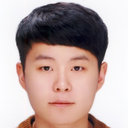
\includegraphics[width=1in,height=1.25in,clip,keepaspectratio]{Jinmyeong-Shin.jpg}}]{Jinmyeong Shin}  received the B.S. degree and Ph.D. degree from Pusan National University, Busan, Republic of Korea, in 2017 and 2024, respectively. From September 2024 to present, he has been a Researcher with Cloud Security Research Center, Pusan National University. He is currently a Visiting Scholar in the Department of Computer Science and Engineering at the University of California, Merced, USA. Dr. Shin’s research interests include privacy-preserving machine learning, vision transformer–based security, differential privacy, and AI-enhanced cryptography.
\end{IEEEbiography}


\begin{IEEEbiography}[{
\includegraphics[width=1in,height=1.25in,clip,keepaspectratio]{prof.jpg}}]{Yoon-Ho Choi}(Member, IEEE) received the M.S. and Ph.D. degrees from Seoul National University, Seoul, South Korea, in 2004 and 2008, respectively. From September 2008 to December 2008, he was a Postdoctoral Scholar with Seoul National University. From January 2009 to December 2009, he was a Postdoctoral Scholar with The Pennsylvania State University, University Park, PA, USA. While working as a Senior Engineer with Samsung Electronics, from May 2010 to February 2012, he was deeply involved in the development of a commercial long-term evolution cloud communication system. He was
an Assistant Professor with Kyonggi University, Suwon, South Korea, from May 2012 to August 2014. He is currently a Professor with the School of Computer Science and Engineering, Pusan National University, Busan, South Korea. His research interests include AI security, privacy preserving
machine learning algorithms, adversarial deep learning, blockchain, deep packet inspection, and anomaly detection algorithms. He served as a member of several technical program committees in various international conferences and journals.
\end{IEEEbiography}

\EOD

\end{document}
